% !TeX spellcheck = it_IT
\section{Algoritmi Paralleli}

Possono essere affrontate 3 diverse problematiche:
\begin{itemize}
	\item \textbf{Sintesi:} progettazione degli algoritmi 
	\item \textbf{Valutazione:} delle prestazioni degli algoritmi
	\item \textbf{Universalità:} quali problemi sono efficientemente risolubili e quali no
\end{itemize}

\paragraph{Sintesi:} Come costruire algoritmi paralleli? Ci si può ispirare ad algoritmi sequenziali, ma quasi mai si può riciclare l'intero algoritmo.\\

\textbf{Esempio}: sommare due numeri binari. L'algoritmo sequenziale ottimo somma i bit per colonna.\\

Porta a un buon algoritmo parallelo? Ogni processore si può occupare di una colonna.\\
Sorge un problema con il riporto, il quale sostanzialmente fa tornare l'algoritmo a uno sequenziale, con in più uno spreco ingiustificato di hardware (ogni processore deve aspettare quello prima...).\\
Ma esistono algoritmi paralleli efficienti per sommare numeri binari.\\

\textbf{Esempio 2}: ordinamento. L'algoritmo sequenziale ottimo è il MergeSort.\\\

Ma questo non porta a un buon algoritmo parallelo, mentre esistono algoritmi paralleli efficienti per l'ordinamento.\\

\textbf{Servono nuove tecniche} e punti di vista totalmente diversi da quelli usati per gli algoritmi sequenziali.\\

\newpage

\paragraph{Valutazione delle prestazioni:} Come si misurano le prestazioni degli algoritmi paralleli? Vanno definiti:
\begin{itemize}
	\item \textbf{Tempo impiegato}
	\item \textbf{Hardware occupato} $=$ numero di processori
\end{itemize}

\textbf{Cos'è efficiente} nel caso di \textbf{algoritmi paralleli}?\\
Si ha un \textbf{parametro} $E= $ \textbf{efficienza}. 	Tiene conto sia del tempo, sia del numero di processori, permettendoci di dire se l'uso aggiuntivo di hardware è giustificato o meno.\\

\paragraph{Universalità:} Si tratta di una problematica teorica, riesco a caratterizzare la classe dei problemi che ammettono algoritmi paralleli efficienti?\\

Nel caso sequenziale la classe di problemi si chiama $\mathcal{FP}$. Nel caso parallelo si \textbf{definisce la classe} $\mathcal{NC}$.\\

$\mathcal{NC} = $ coincide con problemi risolti da algoritmi paralleli efficienti, ovvero con:
\begin{itemize}
	\item \textbf{Tempo polilogaritmico} (quindi meglio che polinomiale, altrimenti userei un algoritmo sequenziale efficiente, dato anch'esso sarebbe polinomiale).\\
	\item \textbf{Hardware polinomiale} (richiede un numero di processori che scala polinomialmente con la lunghezza dell'input).\\
\end{itemize}

Esempi di problemi in $\mathcal{NC}$: 
\begin{itemize}
	\item somma di due numeri
	\item ordinamento 
\end{itemize}

In realtà è ragionevole una sottoclasse di $\mathcal{NC}$, come per $\mathcal{P}$, se il grado del polinomio o le costanti nascoste sono alte, il tempo è sì polinomiale ma rimane poco pratico.\\

\newpage

Si può \textbf{dimostrare che} $\mathcal{NC} \subseteq \mathcal{FP}$.\\
I problemi che possiamo parallelizzare efficientemente rientrano nella classe di problemi risolvibili con algoritmi di calcolo sequenziali efficienti.\\

Per dimostrarlo: per ottenere un algoritmo sequenziale a partire da uno parallelo basta eseguire le istruzioni, che nel parallelo sono divise su vari processori, in fila su un processore singolo, mantenendo il tempo polinomiale (tempo polilogaritmico moltiplicato per il numero polinomiale dei processori, quindi dominato ancora da un polinomiale) e ottenendo un algoritmo sequenziale.\\

Ci si può chiedere se $\mathcal{NC} = \mathcal{FP}$, ma è un problema aperto.\\
Si pensa di no, la questione riprende il problema "ogni algoritmo sequenziale efficiente è parallelizzabile?" Esiste un metodo per trasformare ogni algoritmo sequenziale in un algoritmo parallelo?\\

Se $\mathcal{NC} \neq \mathcal{FP} \implies \mathcal{FP} \setminus \mathcal{NC} = $ problemi $\mathcal{P}-$completi; esistono problemi in $\mathcal{P}$ ma non in $\mathcal{NC}$, chiamati problemi $\mathcal{P}-$completi, problemi tali che la loro appartenenza a $\mathcal{NC}$ farebbe collassare $\mathcal{NC}$ e $\mathcal{FP}$ (ovvero $\mathcal{NC} = \mathcal{FP}$; un problema $\mathcal{P}-$completo permetterebbe di risolvere tutti gli altri problemi di $\mathcal{FP}$, facendo coincidere le due classi).\\

Pertanto non sarò possibile parallelizzare i problemi $\mathcal{P}-$completi (duh).\\
L'universalità non sarà tratta ulteriormente in questo corso.\\

% End of L2

Nel mondo parallelo bisogna: 
\begin{itemize}
	\item fissare un modello di calcolo teorico da mappare su architetture reali
	\item fissare le risorse computazionali, ovvero tempo e numero di processori 
	\item Fissare il parametro efficienza, per dire se una soluzione parallela è preferibile ad una efficiente soluzione sequenziale 
\end{itemize}

\newpage

\subsection{Tipi di architetture parallele}
Ci sono due tipologie:
\begin{itemize}
	\item a \textbf{memoria condivisa}
	\item a \textbf{memoria distribuita}
\end{itemize}

\paragraph{Memoria condivisa:} Ci sono dei processori che si affacciano su una \textbf{memoria centrale condivisa tra tutti}. Si ha un \textbf{clock centrale}.\\
La \textbf{comunicazione avviene in tempo costante}: avendo due processori $P_i$ e $P_j$, $P_j$ vuole comunicare un dato $x$ a $P_i$
\begin{itemize}
	\item $P_j$ scrive $x$ in memoria centrale
	\item $P_i$ legge $x$ dalla memoria centrale
\end{itemize}

In questo modo in 2 cicli di clock avviene la comunicazione. Si dice "comunicazione costante" perché non importa la dimensione del dato da trasferire. Questa è l'attuale architettura di CPU multicore. \\

Questa architettura permette una \textbf{forte parallelizzazione}, dato che i tempi di comunicazione sono trascurabili, rimuovendo quindi il costo dovuto alla comunicazione (o comunque se considerato, è minimo).\\

\paragraph{Memoria distribuita:} Da non confondere con "architetture distribuite", questa è un'architettura parallela a memoria distribuita.\\
Si ha sempre un unico \textbf{clock centrale}, processori sincroni, ma \textbf{ognuno di questi ha una memoria privata} e sono \textbf{collegati tra loro} tramite fili (con qualche topologia, solitamente non fully connected), si ha una \textbf{rete di interconnessione tra i processori}.\\

La comunicazione dipende dalla "distanza" tra i processori: se $P_j$ vuole comunicare $x$ a $P_i$ dobbiamo chiederci quanti processori collegano $P_j$ a $P_i$. Se sono collegati direttamente allora il tempo è costante.\\

La rete di interconnessione è fissa, può essere: 
\begin{itemize}
	\item \textbf{array lineare}: processori collegati su una linea
	\item \textbf{mesh}: collegati su una matrice, sia per riga che per colonna
	\item \textbf{ipercubo}: come prima, ma aumentando le dimensioni
\end{itemize}

\newpage

\subsubsection{PRAM}
\label{subsubsec:PRAM}
Parallel RAM, sta ad indicare che si hanno \textbf{RAM (Random Access Machine) che lavorano in parallelo}, si tratta di un modello teorico ma in pratica lo si ritrova nelle CPU multicore.\\

Si ha un \textbf{determinato numero di processori} ed una \textbf{memoria centrale} $M$, la quale $i-1$esima cella viene indicata con $M[i]$.\\
All'inizio contiene l'input, alla fine può contenere l'output (che può anche essere in uno dei processori).\\

Ogni processore è una RAM ($=$ Random Access Machine) sequenziale e mettendole assieme queste possono lavorare in parallelo.\\
Ogni processore è costituito da una unità di calcolo e dei registri, i quali costituiscono la memoria privata del processore, chiamati $R[0], R[1], ...$.\\

Tipi di istruzioni dei processori $P_i$:
\begin{itemize}
	\item Operazioni aritmetico/logiche.\\
	
	\item Istruzioni da/per la memoria centrale
	\begin{itemize}
		\item  \texttt{store} $R[k]$ $M[h]$: mette il dato nella memoria centrale 
		\item \texttt{load} $R[k']$ $M[h']$: carico nel registro dati dalla memoria centrale alla memoria privata
	\end{itemize}
\end{itemize}
Un processore non può usare i dati $x$ e $y$ se questi sono in memoria centrale, vanno prima caricati nella memoria privata (la ALU è collegata solo ai registri). \textbf{Ogni processore può effettuare operazioni solo sulla propria memoria privata}.\\

Esempio $P_j$ vuole comunicare a $P_i$ il contenuto di $R[t]$. Istruzioni: 
\begin{center}
	\begin{tabular}{c c c}
		$P_j:$ & \texttt{store} & $R[t]$ $M[x]$ \\
		$P_i:$ & \texttt{load} & $R[s]$ $M[x]$
	\end{tabular}
\end{center}
Ovviamente sia \texttt{store} che \texttt{load} devono lavorare sulla stessa cella $M[x]$ della memoria centrale. \\

La comunicazione avviene in tempo $O(1)$.\\

Come si programma con una PRAM?  Si ha un \textbf{unico programma} per tutti i processori ed una \textbf{memoria condivisa}: 
\begin{enumerate}
	\item Il tempo per ogni $P_i$ è scandito dal clock centrale
	\item Ogni $P_i$ esegue la "stessa istruzione"
\end{enumerate}

Cosa si intende con "la stessa istruzione"? Forma dell'istruzione:
\begin{lstlisting}[escapeinside={(*}{*)}]
	for all (*$i \in I$*) par do
		istruzione(*$_i$*)
\end{lstlisting}


Con $I$ definito come l'insieme di indici dei processori che devono eseguire quella istruzione. Si ha un \texttt{for} parallelo, quindi tempo costante  e non $n$ passi diversi, ogni istruzione è indicizzata con l'indice del processore.\\

I processori con indice in $I$ eseguono \texttt{istruzione}$_i$. I processori con indice NON in $I$ eseguono l'istruzione nulla.\\

Cosa si intende con "\texttt{istruzione}$_i$"? Dipende dal tipo di architettura: 
\begin{itemize}
	\item \textbf{SIMD}: Single Instruction Multiple Data
	\item \textbf{MIMD}: Multiple Instruction Multiple Data
\end{itemize}

\paragraph{SIMD:} L'istruzione eseguita è la \textbf{stessa per ogni processore} $\in I$, ma ognuno di questi la effettua \textbf{su dati diversi}.\\

In funzione della \textbf{capacità di accedere alla memoria} $M$ si possono avere più architetture: 
\begin{enumerate}
	\item \textbf{EREW:} Exclusive Read Exclusive Write, scrittura e lettura sono esclusivi, quindi una stessa cella di memoria può essere letta o scritta da un solo processore per volta
	\item \textbf{CREW:} Concurrent Read Exclusive Write, la lettura può essere simultanea, la scrittura è esclusiva
	\item \textbf{CRCW:} Concurrent Read Concurrent Write, lettura e scrittura possono essere simultanee
\end{enumerate}

\newpage

Per la \textbf{scrittura simultanea servono politiche di accesso} (se più processori vogliono scrivere sulla stessa cella, chi vince?): 
\begin{itemize}
	\item \textbf{common:} i processori possono scrivere solo lo stesso dato, pena l'arresto del sistema
	\item \textbf{random:} si sceglie un $P_i$ a caso 
	\item \textbf{max/min:} vince il $P_i$ con il dato max/min
	\item \textbf{priority:} vince il $P_i$ con priorità massima (più alta, va definita una priorità)
\end{itemize}

Indicando con i numeri 1,2,3 le architetture come sopra
$$ Alg(1) \implies Alg(2) \implies Alg(3)$$
Ovvero un algoritmo EREW funziona su architetture CREW, ed un CREW funziona su architetture di tipo CRCW. Questo è abbastanza ovvio, ma vale il contrario? Di base no, ma si possono trasformare CRCW in CREW ed eventualmente anche EREW.\\

L'architettura più ragionevole e più semplice è EREW.\\

Esempio di algoritmo su PRAM di tipo CREW:
\begin{itemize}
	\item numero di processori $=n$
	\item dimensione input $=n$ (lunghezza dell'input pari al numero di processori)
	\item assumiamo input array $A$ con valori distinti
\end{itemize}

Volendo cercare in $A$ un valore particolare:
\begin{lstlisting}[escapeinside={(*}{*)}]
	Cerca (A, n, x) {
		indice=-1
		for (*$i$*)=0 to n-1 pardo 
			P(*$_i$*): 
				if A[i]=x then 
					indice=i
		return indice
	}
\end{lstlisting}

\newpage

Ogni processore di carica nella memoria locale il un dato di \texttt{A} e lo confronta con il valore \texttt{x} cercato (il processore 1 controlla la cella 1, il 2 la cella 2, ...). La variabile \texttt{indice} parte \texttt{=-1}, ma viene settato quando trovato il valore corretto, restituito alla fine.\\

Si ha tempo parallelo e costante. Quanti clock sono? Vanno effettuati: \texttt{load x}, \texttt{load A[i]}, il confronto ed eventualmente la scrittura della variabile indice, quindi $4$ cicli di clock.\\

Questo algoritmo è concurrent read perché la \texttt{x} viene letta assieme da tutti, mentre su \texttt{A} vengono lette sempre celle diverse. Exclusive write perché la scrittura invece viene effettuata da un solo processore, solo quando viene scritto l'indice, con il presupposto che \texttt{A} contenga solo valori distinti.\\

Se \texttt{A} può contenere elementi ripetuti allora questo algoritmo diventa CRCW, dato che posso trovare più valori pari a \texttt{x} tutti nello stesso momento.\\

\paragraph{Risorse di calcolo:}
\begin{itemize}
	\item nel \textbf{sequenziale}: $t(n)$ (tempo), $s(n)$ (spazio)
	\item nel \textbf{parallelo}: $p(n)$ (numero di processori), $T(n, p(n))$ (tempo, in funzione di input e numero di processori)
\end{itemize}

Definizioni informali: 
\begin{itemize}
	\item $p(n)$: numero di processori richiesti su input di lunghezza $n$ (nel caso peggiore)
	\item $T(n, p(n))$: tempo richiesto da un input di lunghezza $n$ su $p(n)$ processori. Di conseguenza $T(n, 1)$ è il tempo sequenziale 
\end{itemize}

%mancano le ultime due slide

%Fine L3

%Videolezione, partendo dalla fine della 3, poi 4

\newpage

\paragraph{Valutazione precisa del tempo $T(n, p(n))$:} Possiamo pensare all'esecuzione del programma con una sorta di matrice con: 
\begin{itemize}
	\item colonne che rappresentano ognuna uno dei $p(n)$ processori
	\item righe che rappresentano ognuna un passo parallelo 
\end{itemize}
Quindi nella prima riga ho il primo passo parallelo e sotto la prima colonna avrò l'istruzione eseguita dal primo processore.\\

Il numero dei passi generalmente dipende da $n$, per cui diventa una funzione $k(n)$.\\

Il costo, in termini di tempo, per il primo processore al primo step del programma viene indicato con $t_1^{(1)} (n)$, dove la $t$ è piccola perché è un tempo sequenziale, all'apice si trova il numero del processore e al pedice il numero del passaggio.\\

Vogliamo \textbf{definire} $T(n, p(n))$ \textbf{in funzione} di questi \textbf{tempi richiesti dalle singole RAM}, ovvero la \textbf{somma dei tempi richiesti da ognuno dei $k(n)$ passi}. Supponendo un'architettura MIMD, istruzioni diverse potrebbero richiedere tempo diverso, quindi a \textbf{ogni passo dobbiamo considerare il tempo massimo} impiegato da un singolo processore; il massimo per ogni riga, per ogni $t_1$.\\
Indichiamo il tempo impiegato al passo $i$-esimo con
$$ t_i (n) = \max \left\{ t_i^{(j)} (n) | \, 1 \leq j \leq p(n) \right\}$$
Di conseguenza: 
$$ T\left(n, p(n)\right) = \sum_{i = 1}^{k(n)} t_i (n) $$
Il \textbf{tempo parallelo} è la somma del tempo a ogni passaggio:
\begin{itemize}
	\item $T$ \textbf{dipende da} $k(n)$ (devo sommare $k(n)$ passi)
	\item $T$ \textbf{dipende anche dalla dimensione dell'input} (costo logaritmico/uniforme, il tempo sequenziale a ogni passo dipende dalla dimensione dell'input in quanto elaborato da macchine sequenziali)
	\item $T$ \textbf{dipende da} $p(n)$ (le operazioni da eseguire sono sempre quelle, se i processori sono troppo pochi devo assegnare le operazioni rimanenti in coda ad altre su altri processori; eventualmente alcuni processori in un solo step dovranno svolgere più operazioni)
\end{itemize}

\newpage

\subsection{Broadcast P-RAM}

Al posto di processori consideriamo entità, che collaborano tra loro ed una informazione $i$, detenuta da una sola entità, deve essere conosciuta da tutte le altre entità che compongono il sistema. Broadcast o replica, si ha un array in memoria centrale/condivisa in cui \textbf{una cella contiene il valore} $x$ e vogliamo che \textbf{nelle celle seguenti compaia il valore} $x$ \textbf{per un certo numero di elementi} $n$, in modo che gli altri processori possano conoscere l'informazione nella loro cella associata. Le celle della memoria condivisa vengono indicate come $A$. 

\begin{lstlisting}[escapeinside={(*}{*)}]
	Broadcast ((*$x$*))
	{
(*$P_0:$*)	A[(*$0$*)] = (*$x$*)
	for (*$i=0$*) to (*$\log n - 1$*) do
		for (*$j=2^i$*) to (*$2^{i+1}-1$*) par do
(*$P_j$:*)		A[(*$j$*)] = A[(*$j - 2^i$*)]
	}
\end{lstlisting}

Per la condivisione ci sono $\log n$ passi paralleli, un certo numero di processori prendono il valore $x$ e lo copiano in una delle celle successive (ogni processore lo passa ad un'altra cella, raddoppiando il numero di celle contenenti $x$ ogni volta e ripetendo), rendendo il numero di passaggi richiesti logaritmico rispetto al numero $n$ di copie dei dati da avere.\\

Questo processo potrebbe essere eseguito perché in un programma EREW ogni processore deve accedere ad una sua copia del dato non avendo letture concorrenti. \\

\newpage

Il broadcast può essere usato per risolvere \textbf{la ricerca}:
\begin{lstlisting}[escapeinside={(*}{*)}]
	Cerca ((*$a,n,x$*))
	{
		Broadcast((*$x$*))
		Indice=(*$-1$*)
		for (*$i=0$*) to (*$n-1$*) par do
(*$P_i:$*)			if A[(*$i$*)]=x[(*$i$*)] then indice=(*$i$*)
		return indice
	}
\end{lstlisting}

Faccio il broadcast del dato $x$ e lo faccio cercare da tutti i processori, restituendo l'indice $i$ del dato, se trovato. Di conseguenza impiega tempo $\log n$ (solamente $1$ passo per la ricerca, $\log n$ per il broadcast).\\

Se tutti gli indici sono distinti l'algoritmo è EREW, altrimenti ERCW (ma solitamente si usa solo CRCW, non ha senso avere scritture concorrenti e letture esclusive). ERCW può essere trasformato in EREW (con un aumento della funzione tempo).\\

\newpage

\subsection{Efficienza}
Per progettare algoritmi paralleli è necessario stabilire cosa significhi in questo contesto "buone prestazioni", in modo da essere sicuri che questi migliorino effettivamente gli algoritmi sequenziali. \\

Bisogna valutare la funzione tempo dell'algoritmo parallelo $T(n, p(n))$ in confronto al tempo sequenziale $T(n,1)$: se il tempo parallelo ha un tasso di crescita migliore di quello sequenziale allora l'algoritmo parallelo ha migliorato la soluzione.\\
Per il confronto tra i due tempo ci sono due possibilità:
\begin{itemize}
	\item Il tempo \textbf{parallelo} è \textbf{circa uguale} al tempo \textbf{sequenziale}
	$$ T(n, p(n)) = \Theta(T(n,1))$$
	Il tempo parallelo è limitato sia superiormente che inferiormente dal tempo sequenziale, \textbf{stesso tasso di crescita}. Questo è il caso \textbf{da evitare}. Il confronto dei tempi tramite parametro efficienza esclude la possibilità di ricadere in questo caso.\\
	
	\item Il tempo \textbf{parallelo cresce più lentamente} del \textbf{tempo sequenziale}
	$$ T(n, p(n)) = o (T(n,1))$$
	Viene \textbf{limitato superiormente} (in qualche modo) dal \textbf{tempo sequenziale}, la funzione del tempo parallelo è sempre più piccola di quello sequenziale. Questo è il caso \textbf{da preferire}, il parametro efficienza vuole questa situazione.\\
\end{itemize}

\newpage

\subsubsection{Speed-up}
Parametro che serve a definire l'efficienza, si tratta del \textbf{rapporto tra il tempo sequenziale per risolvere il problema e il tempo richiesto dall'algoritmo parallelo}:
$$ S(n, p(n)) = \frac{T(n,1)}{T(n,p(n))} $$
Esempio: se $S=4$ l'algoritmo parallelo è $4$ volte più veloce del sequenziale.\\

Ma in realtà se desse 4 sarebbe un caso in cui il parallelo è un $\Theta$ del sequenziale. Ponendoci nel \textbf{caso in cui} $T(n, p(n)) = o (T(n, 1))$ lo speed-up \textbf{tende a infinito}
$$ S(n, p(n)) \rightarrow + \infty $$

Con un rapporto dei tempi (questo parametro), viene considerato il numero di processori? In realtà no, \textbf{non considera il numero di processori}, potremmo averne utilizzata una quantità troppo elevata/non vantaggiosa, ma questo parametro non fornisce modo di saperlo, sappiamo il rapporto tra i tempi ma non riusciamo a considerare se il numero di processori è adeguato.\\
Per questa mancanza, il parametro di speed-up viene poi \textbf{usato solamente per definire il parametro efficienza}. \\

\paragraph{Esempio di un problema:} Soddisfacimento di formule (dove la lunghezza della formula è legata linearmente al numero di variabili coinvolte); si tratta di un problema $\in \mathcal{NP}$:
$$ T(n,1) = 2^n$$
Utilizzando un processore per ogni possibile assegnamento (sostanzialmente il funzionamento di una macchina non deterministica): 
$$ T(n, p(n)) = O(n) $$
$$S(n, p(n)) = \frac{2^n}{n} \rightarrow +\infty \;\text{ ma }\; p(n) = 2^n$$
Tecnicamente lo speed-up tende a infinito, ma il numero di processori è decisamente non polinomiale, costo hardware esponenziale.

\newpage

\subsubsection{Definizione di Efficienza}
Il parametro efficienza è definito come il \textbf{rapporto tra lo speed-up e il numero di processori $p(n)$}
$$ E(n, p(n)) = \frac{S(n,p(n))}{p(n)} = \frac{T(n,1)^\ast}{p(n) \cdot T(n, p(n))}$$

Viene usato $T(n,1)^\ast$, ovvero il miglior tempo sequenziale conosciuto per risolvere il problema o un lower bound di quest'ultimo, giusto per essere più cattivi con il nostro algoritmo parallelo.\\

Il parametro efficienza \textbf{può assumere i valori}
$$ 0 \leq E(n, p(n)) \leq 1$$
Che sia sempre $\geq 0$ lo si vede dalla formula, essendo un rapporto tra valori sempre positivi.\\

Esempio per il problema di soddisfacimento di formule:
$$ E(n, p(n)) = \frac{2^n}{2^n \cdot n} = \frac{1}{n} \rightarrow 0 $$

\paragraph{Principio di Wyllie:} Quando l'\textbf{efficienza tende a 0} $E \rightarrow 0$, l'\textbf{utilizzo di processori è troppo elevato}, che magari rimarranno utilizzati la maggior parte del tempo.\\

Che l'efficienza sia sempre $\leq 1$ invece lo si può intuire dal fatto che è un rapporto tra tempo sequenziale e tempo parallelo moltiplicato per numero di processori. Portato all'estremo, ipotizzando di poter usare $n$ processori per risolvere in 1 passo un problema con input $n$ il tempo sequenziale dello stesso algoritmo diventerebbe $n$ (mettere tutti i passi uno dopo l'altro), il numero di processori è $n$ mentre il tempo parallelo sarà 1, quindi diventa $n/n$ (inventato da me, sotto spiegazione un po' più formale). \\

\newpage

Per dimostrarlo, chiamo $\tilde{T} (n, 1)$ la versione sequenziale dell'algoritmo parallelo (tutti i passaggi svolti in fila), di conseguenza 
$$ T(n, 1) \leq \tilde{T} (n,1) \leq p(n) t_1 (n) + p(n) t_2 (n) + \, ... \, + p(n) t_{k(n)} (n) $$
l'algoritmo sequenziale "normale" è sicuramente $\leq$ del nostro $\tilde{T}$, che impiega al massimo la somma del tempo di ogni passaggio moltiplicato per il numero di processori, ma questa è la definizione del tempo parallelo.\\
$$ p(n) t_1 (n) + p(n) t_2 (n) + \, ... \, + p(n) t_{k(n)} (n) = p(n) \sum_{i = 1}^{k(n)} t_i (n) = p(n) T(n, p(n)) $$

Il miglior tempo sequenziale è limitato superiormente dal miglior tempo parallelo moltiplicato per il numero di processori
$$ T(n,1) \leq p(n) \cdot T(n, p(n)) $$
E da qua possiamo ricavare
$$ \frac{T(n,1)}{p(n)} \leq T(n, p(n))$$
Il tempo parallelo $T(n, p(n))$ ha un lower bound, ovvero il rapporto tra il miglior tempo sequenziale e il numero di processori. Il meglio che posso fare con un algoritmo parallelo è distribuire equamente il lavoro tra tutti i processori.\\

Spostando anche il tempo parallelo nella disequazione si ottiene 
$$ \frac{T(n,1)}{p(n) T(n, p(n))} \leq 1 \implies E(n, p(n)) \leq 1$$
l'efficienza è $\leq 1$.\\

Di conseguenza l'\textbf{efficienza è un parametro che varia tra 0 e 1}: 
\begin{itemize}
	\item Se $E \rightarrow 0$ non va bene: implica che $p(n)$ cresce troppo velocemente, dato che $T(n, p(n)) = o(T(n,1))$
	\item Il meglio da avere è $E \rightarrow k \leq 1$ dove $k$ è una costante
\end{itemize}

\newpage

Altro modo per dimostrare che $E \leq 1$, basandosi sull'idea che se $E \rightarrow 0$ allora per migliorare l'algoritmo provo a ridurre $p(n)$ senza degradare il tempo. Cambio il numero di processori da $p$ a $p/k$.\\

Ricetta presa dalla PhD thesis di J. Wyllie.\\

Su un algoritmo generico, ridurre i processori a $p/k$ significa che a ogni passo ogni processore deve svolgere in sequenza le operazioni di $k$ processori, sostanzialmente vengono raggruppate le operazioni $k$ alla volta. Il tempo di ogni passo sarà limitato superiormente da $k \cdot t_i(n)$ ($k$ il tempo di ogni passo, sicuramente sarà maggiore in quanto il tempo di ogni passo è definito come il $\max$ di tutti).\\

Il tempo parallelo richiesto dall'algoritmo con $p/k$ processori è limitato superiormente dalla somma dei tempi all'$i$-esimo passo: 
$$ T(n, p/k) \leq \sum_{i = 1}^{k(n)} k \cdot t_i (n) = k \cdot \sum_{i = 1}^{k(n)} t_i (n) = k \cdot T(n, p) $$
Quindi si ha che 
$$ T(n, p/k) \leq k \cdot T(n, p)$$
Di conseguenza il tempo con $p/k$ processori è limitato superiormente dal tempo che usa tutti i $p$ processori, moltiplicato per $k$.\\

Partendo da questa disuguaglianza si può far vedere che \textbf{l'efficienza $E$ cresce al diminuire dei processori}.\\

\newpage

\textbf{Quanto vale} $E \left(n, p/k\right)$?
$$ E \left(n, p/k\right) = \frac{T(n,1)}{\frac{p}{k}  \cdot T(n,p/k)} \geq \frac{T(n,1)}{\frac{p}{k} \cdot k \cdot T(n,p)} = E(n,p) $$
%Slide
Sostituisco $T(n, p/k)$ con $k \cdot T(n, p)$ (ricordando che $T(n, p/k) \leq k \cdot T(n, p)$). Abbiamo sostituito un valore più grande, dividendo per un valore più grande ottengo un valore più piccolo, quindi la disuguaglianza diventa $\geq$.

$$ E(N, p/k) \geq E(n,p) $$

La formula mostra che \textbf{diminuendo i processori migliora il parametro efficienza} (aumenta, rendendo vera la ricetta di Wyllie). Se il miglioramento è significativo è un altro discorso.\\

Considerando $k \rightarrow p$
$$ 1 = E(n,1) = E(n, p/p) \geq E(n, p/k) \geq E(n,p) $$

Quindi si ottiene l'efficienza di un algoritmo sequenziale. Attenzione a mantenere $T(n, p/k) = o(T(n,1))$ (perché $E(n,1) = 1$, ma $T(n, p=1) = T(n,1)$ cioè sequenziale).\\

\newpage

\subsection{Problema Sommatoria}
Perché prendiamo esempi di problemi? Motivazioni:
\begin{itemize}
	\item \textbf{Tecnica:} scomposizione del problema in sottoproblemi e fusione dei risultati
	\item \textbf{Schema:} "imparando" la sommatoria posso adattare la soluzione per altre operazioni associative
	\item \textbf{Modulo:} sotto-problema di altri problemi più grandi 
\end{itemize}

Problema della sommatoria: 
\begin{itemize}
	\item \textbf{Input:} $M[1], M[2], ... , M[n]$, $n$ elementi in $n$ celle della memoria
	\item \textbf{Output:} $M[n] = \sum_{i=1}^n M[i]$, nell'ultima cella verrà scritta la somma di tutti i valori (presupponendo non sia importante mantenere le informazioni preesistenti nelle celle)
\end{itemize}

Algoritmo sequenziale: 
\begin{lstlisting}[escapeinside={(*}{*)}]
	for (*$i=1$*) to (*$n-1$*) do:
		M[(*$n$*)] = M[(*$n$*)] + M[(*$i$*)]
\end{lstlisting}
Accumulo tutto in $M[n]$ sequenzialmente. Il tempo diventa $T(n,1) = n-1$ passaggi.\\

L'idea per parallelizzare è \textit{"una somma a processore"}: somme a due a due, ogni processore somma una coppia di valori e ripeto il processo fino ad ottenere la somma finale. Servono quindi $\log n$ passi per sommare $n$ elementi.\\

Questo \textbf{funziona }solo \textbf{perché} il $+$ è \textbf{associativo}:
$$ ((a+b) + c) + d = (a+b) + (c+d)$$
Quindi questo \textbf{schema può essere applicato ad ogni altra operazione associativa}.\\

\newpage

Al primo passo sommo elementi a distanza 1, al secondo passo distanza 2, al terzo passo distanza 4, ..., all'ultimo passo rimarranno 2 valori da sommare a distanza $n/2$; la distanza raddoppia ad ogni passo. Ogni risultato parziale viene memorizzato nella cella di indice più alto.\\

Istruzioni (con $k=$ numero del processore): 
\begin{center}
	\begin{tabular}{c c c}
		$1^{\circ}$ passo: & \texttt{M[2k] = M[2k] + M[2k-1]} & $1 \leq k \leq \frac{n}{2}$ \\
		$2^{\circ}$ passo: & \texttt{M[4k] = M[4k] + M[4k-2]} & $1 \leq k \leq \frac{n}{4}$ \\
		& ... & \\
		$\log n^{\circ}$ passo: & \texttt{M[n] = M[n] + M[n/2]} & $1$
	\end{tabular}
\end{center}

Pseudo-codice:
\begin{lstlisting}[escapeinside={(*}{*)}]
	for (*$j=1$*) to (*$\log n$*)
		for (*$k=1$*) to (*$n/2^j$*) par do
			M[(*$2^j k$*)] = M[(*$2^j k$*)] + M[(*$2^j k - 2^{j-1}$*)]
	return M[(*$n$*)]
\end{lstlisting}

% Non ha finito le slide
% End L5

\paragraph{Questo algoritmo è EREW?} Dobbiamo valutare se l'\textbf{uso delle celle è esclusivo}, ovvero se ci sono letture/scritture simultanee.\\

Considerando due processori $a,b$ con $a \neq b$, a questo scopo dobbiamo verificare che $2^j a$, $2^j a - 2^{j-1}$, $2^j b$ e $2^j b - 2^{j-1}$ siano tutti diversi tra loro.\\

I confronti possibili quindi sono:
\begin{itemize}
	\item $2^j a \neq 2^j b$, che vale per ogni $a \neq b$
	\item $2^j a \neq 2^jb - 2^{j-1}$ ovvero $2 a = 2b - 1$ e non esistono valori $\in \mathbb{N}$ che soddisfano l'equazione
\end{itemize}

Quindi abbiamo dimostrato che \textbf{è un algoritmo EREW}.

\newpage

\paragraph{Dimostrare la correttezza:} Per la correttezza dobbiamo \textbf{dimostrare la proprietà}:
$$ M[2^j k] = M[2^j k] + \, ... \, + M[2^j (k-1) + 2] + M[2^j (k-1) + 1] $$
Nelle celle multiple di $2^j$ (con $1 \leq j \leq \log n$) ci sono $2^j$ valori sommati, ovvero quelli appartenenti a tutte le $2^j$ celle precedenti.\\

Per $j = \log n$ e di conseguenza $k=1$ la proprietà sopra risulta:
$$ M[n] = M[n] + \, ... \, + M[1] $$
In $M[n]$ ci va la somma degli $n$ precedenti valori.\\

Si può dimostrare \textbf{per induzione}: 
\begin{itemize}
	\item \textbf{Caso base:} $j=1$ e $1 \leq k \leq \frac{n}{2}$. L'istruzione dell'algoritmo è
	$$ M[2k] = M[2k] + M[2k-1] $$
	Quindi per $j=1$ è facile verificare che la proprietà è vera.\\
	
	\item \textbf{Induzione:} si presuppone che la proprietà sia vera per $j-1$ e si dimostra che vale per $j$. Consideriamo l'istruzione del programma al passo $j$
	$$ M[2^j k] = M[2^j k] + M[2^jk - 2^{j-1}]$$
	e dobbiamo dimostrare che questa è in realtà un'istruzione che mette nella cella di memoria $2^j k$ la somma dei suoi precedenti $2^j$ valori.\\
	
	Raccolgo $2^{j-1}$ ottenendo $M[2^{j-1} 2k]$, quindi per la proprietà e per ipotesi induttiva posso dire che:
	$$ M[2^{j-1} 2k] = M[2^{j-1} 2k] + \, ... \, + M[2^{j-1} (2k-1)+1]$$
	Quindi dentro $M[2^{j-1} 2k]$ sono presenti tutti i valori precedenti con un fattore moltiplicativo $(2k-1)$; è uguale alla proprietà iniziale, cambia solo che al posto di $k$ è presente $2k$. Nella cella di indice $2k$ abbiamo la somma di tutti i precedenti $2^{j-1}$ valori.\\
	
	Raccogliendo $2^{j-1}$ anche da $M[2^jk - 2^{j-1}]$ risulta $M[2^{j-1} (2k-1)]$, che come prima può essere visto come un multiplo di $2^{j-1}$, quindi applichiamo ancora la proprietà per ipotesi di induzione:
	$$ M[2^{j-1} (2k-1)] = M[2^{j-1} (2k-1)] + \, ... \, + M[2^{j-1} (2k-2)+1]$$
	Allora abbiamo che la cella $M[2^{j-1} (2k-1)]$ contiene tutte le precedenti $2^{j-1}$ celle.\\
	
	Quindi abbiamo che in $M[2^j k]$ sono contenuti $2^{j-1}$ valori, così come in $M[2^jk - 2^{j-1}]$, ovvero le due celle considerate all'inizio. Il totale degli elementi sommati quindi è $2^{j-1} + 2^{j-1} = 2^j$. Di conseguenza in $M[2^j k]$ vengono sommati $2^j$ valori.\\
	
	Possiamo verificare che siano tutti valori differenti notando che sono tutti valori in sequenze decrescenti, ma l'ultimo della prima uguaglianza e il primo della seconda sono rispettivamente $M[2^{j-1} (2k-1)+1]$ e $M[2^{j-1} (2k-1)]$ ovvero il secondo valore è il successivo del primo.
	
	$$M[2^{j-1} (2k-1)+1] \xLeftrightarrow[\text{precedente}]{\text{successivo}} M[2^{j-1} (2k-1)]$$
	
	Essendo sequenze decrescenti abbiamo verificato che siano tutti i valori diversi, quindi la somma delle due celle racchiude tutti i $2^j$ valori.\\
	
	Di conseguenza
	$$ M[2^j k] = M[2^j k] + \, ... \, + M[2^j (k-1) + 1] $$
	è vera.\\
	
\end{itemize}

\newpage

\subsubsection{Valutazione dell'algoritmo}
\paragraph{Numero di processori:} Il numero di processori impiegati è dato dal livello più "costoso", ovvero il primo, nel quale ne vengono usati $n/2$ (anche se a ogni passo ne verranno usati la metà di quello precedente)
$$ p(n) = \frac{n}{2} $$

\paragraph{Tempo:} Il tempo impiegato deve considerare, oltre al numero di passaggi, le microistruzioni necessarie:
\begin{itemize}
	\item \texttt{LD} per caricare il primo numero
	\item \texttt{LD} per caricare il secondo numero
	\item \texttt{ADD} per sommare i numeri
	\item \texttt{ST} per rimettere il numero in memoria centrale
\end{itemize}
ovvero $4$ operazioni per $\log n$ passaggi, quindi
$$ T(n, n/2) = 4 \log n $$

Se $n$ non è potenza di 2 bisogna allungare l'input con degli $0$ fino ad arrivare al multiplo di 2 successivo ad $n$. Non può peggiorare drasticamente le prestazioni in quanto in binario, chiamando $t$ il numero di bit necessari per rappresentare $n$, la potenza di 2 più vicina ad $n$ diventa $t$ zeri con in testa un 1 e quindi sarà sempre compresa tra $n$ e $2n$. Nel peggiore dei casi l'input si raddoppia. \\

Quindi le valutazioni viste per $n$ potenza di 2 valgono anche nelle altre casistiche, però:
$$ p(n) = \frac{2n}{2} = n $$
$$ T(n,n) = 4 \log 2n \leq 5 \log n$$
$$ \implies p(n) = O(n) \;\;\text{ e } \;\; T(n,n) = O(\log n)$$

\paragraph{Efficienza:} Possiamo calcolare l'efficienza
$$ E(n,n) = \frac{n-1}{n \cdot 5 \log n} \sim \frac{1}{5 \log n} \rightarrow 0 \;\text{ (lentamente)}$$
I processori sono un po' "sprecati", in quanto vengono utilizzati tutti solamente al primo passo.\\

\newpage

Proviamo a vedere se, applicando Wyllie, si può \textbf{diminuire il numero di processori} fino a sub-lineare, quindi con $p(n) = o(n)$, \textbf{mantenendo un tempo logaritmico}, anche con diverso coefficiente. Questo per avere una efficienza che tende ad una costante diversa da zero, $E \rightarrow c \neq 0$. \\

Quindi partendo da $n$ numeri, al posto di avere $n/2$ processori ne abbiamo $p$ (per ora indefinito). Ognuno dei $p$ processori dovrà \textbf{farsi carico di} una certa quantità di \textbf{numeri da sommare} $\Delta = n/p$.\\
Ogni processore effettuerà la somma di $\Delta$ elementi. \\

I \textbf{risultati} verranno messi nella \textbf{cella coinvolta dalla somma} con \textbf{indice più alto}, quindi $M[\Delta], M[2 \Delta], \, ... \, , M[p \Delta]$.\\

Con $k$ indice del processore, $1^\circ$ passo parallelo:
$$ M[k \Delta] = M[k \Delta] + \, ... \, + M[(k-1) \Delta + 1] \;\;\;\;\;\; 1 \leq k \leq p $$
Quindi nella cella $M[k \Delta]$ verrà messa la somma dei $\Delta$ numeri affidati al processore $k$.\\

Passi \textbf{paralleli successivi}: i risultati parziali sono nelle celle
$$ M[\Delta], M[2\Delta], \, ... \, , M[p \Delta] $$
A queste celle applichiamo l'algoritmo sommatoria visto prima, in modo tale che $ M[p \Delta] = M[n] = \sum_i M[i] $, ovvero le somme di tutti i gruppetti parziali.\\
Questo \textbf{dimostra} la \textbf{correttezza} dell'algoritmo.\\

Di conseguenza applico l'algoritmo precedente per la sommatoria alle $p$ somme parziali ottenute. Tempo $n/p$ per il primo passo e $5 \log p$ per i restanti.\\

\newpage

\paragraph{Valutazione:} Per il nuovo algoritmo:
\begin{itemize}
	\item I \textbf{processori} sono
	$$p (n) = p $$
	
	\item Il \textbf{tempo} diventa 
	$$T (n,p) = T(1^\circ \text{ passo }) + T(\text{ passi succ. }) = \frac{n}{p} + 5 \log p$$
\end{itemize}
Di conseguenza l'\textbf{efficienza}
$$ E (n,p) = \frac{n-1}{p\left(\frac{n}{p} + 5 \log p \right)} = \frac{n-1}{n + 5p \log p} \rightarrow c \neq 0 $$
Non abbiamo dato un valore a $p$, ma sarebbe carino se $5p \log p = n$ in modo tale che $n+n$ al denominatore abbatta il tempo sequenziale sopra, \textbf{tendendo a una costante} $c \neq 0$. Presupponendo $5p \log p = n$:
$$ E (n,p) \sim \frac{n}{2n} \rightarrow \frac{1}{2} $$

Per fissare $p$: 
$$ p \log p = \frac{n}{5} \implies p = \frac{n}{5 \log n} $$
e si può facilmente verificare che il valore è corretto.

\paragraph{Ricapitolando:} i valori diventano:
$$ p(n) = \frac{n}{5 \log n} $$
$$ T(n, p(n)) = 5 \log n + 5 \log n - \, ... \, \leq 10 \log n $$
Quindi il numero di processori è sub-lineare, mantenendo il tempo logaritmico, seppur con una diversa costante.

\vfill 

\paragraph{Si può fare di meglio?} Si può migliorare l'algoritmo per la sommatoria? Si può dimostrare un lower bound sfruttando il fatto che un algoritmo per la sommatoria non è altro che un albero binario e può essere sempre rappresentato come tale. Il livello con più nodi determina il numero di processori, mentre l'altezza dell'albero determina il tempo.\\

Di conseguenza \textbf{meglio di} $\log n$ \textbf{non si può fare}.\\

% Fine videolezione 6

\subsubsection{Sommatoria come schema per altri problemi}

Una operazione iterata, con la proprietà di essere associativa:
\begin{itemize}
	\item Input $M[1], \, ... \, , M[n]$
	\item Output $Op_i M[i] \rightarrow M[n]$, ovvero effettuo l'operazione su tutti gli elementi e metto il risultato in $M[n]$
\end{itemize}

Esempi di operazioni associative: $+,\ast,\wedge, \vee,\oplus$.\\

Questo permette di avere una soluzione efficiente parallela: 
$$ p = O \left(\frac{n}{\log n}\right) \;\;\;\;\; T = O(\log n) $$

Con modelli di PRAM più potenti si possono ottenere tempi migliori, fino a costante.\\

\newpage

\paragraph{Problema dell'$\wedge$-iterato:}
$$ M[n] = \bigwedge_i M[i] $$
Programma
\begin{lstlisting}[escapeinside={(*}{*)}]
	for (*$i \leq k \leq n$*) par do 
		if M[(*$k$*)] = 0 then
			M[(*$n$*)] = 0
\end{lstlisting}

Sostanzialmente, mi basta uno 0 ed il risultato diventa 0.\\

Per questo programma però serve un'architettura \textbf{CRCW} (lettura esclusiva in realtà), in quanto potenzialmente \textbf{più processori} dovranno \textbf{accedere} alla \textbf{cella} $M[n]$. Si può usare la politica common.\\

Le \textbf{prestazioni} che ne risultano: 
$$ p(n) = n $$
$$ T(n,n) = 3 $$
$$ E(n,n) = \frac{n-1}{n \cdot 3} \rightarrow \frac{1}{3} $$

Si può usare lo stesso programma per l'\texttt{OR}, basta cambiare 0 con 1 e diventa "basta un 1 per far diventare 1 il risultato".\\

La sommatoria può essere un sottoproblema di altri: 
\begin{itemize}
	\item prodotto interno di vettori: $<... , ...>$ 
	\item prodotto matrice-vettore
	\item prodotto matrice-matrice
	\item potenza di una matrice
\end{itemize}

\newpage

\paragraph{Prodotto interno di vettori:}
\begin{itemize}
	\item Input: $x,y \in \mathbb{N}^n$, due vettori di $n$ elementi
	\item Output: il prodotto interno dei due vettori, $<x,y> = \sum_{i=1}^n x_i \ast y_i$
\end{itemize}
Sono $n$ prodotti e sommarne i risultati, quindi $n-1$ somme, il tempo sequenziale risulta $2n-1$.\\

La soluzione EREW è applicare il \textbf{modulo sommatoria} con in \textbf{input} ad \textbf{ogni processore} un \textbf{gruppo di} $\Delta = n/p$ coppie di $x_i \ast y_i$ (sommatoria parallela con la riduzione dei processori descritta prima).\\

\begin{itemize}
	\item Fase \RNum{1}: $\Delta$ prodotti in sequenza per processore e somma sequenziale
	\item Fase \RNum{2}: somma di $p$ numeri in parallelo
\end{itemize}

Per la sommatoria (Fase \RNum{2}) serve un numero di processori: 
$$ p = c_1 (\frac{n}{\log n}) \;\;\;\;\; t_{II} = c_2 \log n $$

Mentre per la Fase \RNum{1}: 
$$ p \sim \frac{n}{\log n}  \implies \Delta = \frac{n}{p} = \log n \implies t_{I} = c_3 \log n$$

Riassumendo:
$<x,y>$ \textbf{costa}: $p(n) \sim \frac{n}{\log n}$, $t = t_{I} + t_{II} \sim \log n$, quindi:
$$ E \sim \frac{2n-1}{\frac{n}{\log n} \cdot \log n} \rightarrow c \neq 0 $$

Ci sono costanti non riportate, viene un numero minore di 1 ovviamente.\\

\newpage

\paragraph{Prodotto matrice vettore:}
\begin{itemize}
	\item Input: una matrice $A \in \mathbb{N}^{n \times n}$ ed un vettore $x \in \mathbb{N}^n$
	\item Output: il prodotto tra i due $Ax$ 
\end{itemize}

Ognuna delle $n$ \textbf{righe} della matrice $A$ viene \textbf{moltiplicata per il vettore}, quindi sono necessarie $n(2n-1) = 2n^2 -n$ operazioni (ognuna delle $n$ righe della matrice è un vettore moltiplicato per un altro, quindi $n$ volte il prodotto vettoriale).\\

Sapendo già come fare il prodotto interno, si può usare il modulo di quest'ultimo in parallelo $n$-volte per risolvere il prodotto matrice-vettore.\\

Il vettore $x$ è acceduto simultaneamente dai moduli per il prodotto interno $\implies$ algoritmo CREW.\\

Le \textbf{prestazioni} che ne risultano: 
$$ p(n) = n \cdot \frac{n}{\log n} \;\;\;\;\; T(n, p(n)) \sim \log n $$
$$ E (n, p(n)) \sim \frac{n^2}{\frac{n^2}{\log n} \cdot \log n} \rightarrow c \neq 0$$

\newpage

\paragraph{Prodotto matrice matrice:} 
\begin{itemize}
	\item Input: due matrici $A,B \in \mathbb{N}^{n \times n}$
	\item Output: il prodotto $A \times B$
\end{itemize}

Si può risolvere usando $n^2$ \textbf{prodotti interni in parallelo}.\\

Tempo sequenziale: $n^{2.8}$ (Strassen), oppure $n^{2.37}$ (Le Gall 2014)

Ogni riga di $A$ e colonna di $B$ vengono accedute simultaneamente $\implies$ algoritmo CREW. La lettura concorrente si potrebbe eliminare usando un broadcast dei dati.\\

Le \textbf{prestazioni} che ne risultano: 
$$ p(n) \sim n^2 \cdot \frac{n}{\log n} \;\;\;\; T(n, p(n)) \sim \log n $$
$$ E(n, p(n)) \sim \frac{n^{2.8}}{\frac{n^3}{\log n} \log n} = \frac{n^{2.8}}{n^3} \rightarrow 0 \;\;(\text{lentamente}) $$ 
Anche se lentamente, tende a zero, quindi in questo modo non è considerato efficiente.\\

\newpage

\paragraph{Potenza di matrice:}
\begin{itemize}
	\item Input: una matrice $A \in \mathbb{N}^{n \times n}$
	\item Output: $A^n$ con $n = 2^k$
\end{itemize}

Si tratta di un \textbf{prodotto iterato} della \textbf{stessa matrice}, quindi posso moltiplicare $A \times A$, poi $A^2 \times A^2$, ecc.; così richiedendo un numero logaritmico di passaggi.\\

Sequenzialmente: 
\begin{lstlisting}[escapeinside={(*}{*)}]
	for (*$i = 1$*) to (*$\log n$*) do
		A = A (*$\times$*) A 
\end{lstlisting}

Tempo sequenziale: $n^{2.8} \cdot \log n$.\\

Per il parallelo: sfrutta la stessa idea del sequenziale, quindi bisogna effettuare $\log n$ volte il prodotto $A \times A$, sostituendo il prodotto sequenziale con quello parallelo. Ovviamente algoritmo CREW.\\

Le \textbf{prestazioni} che ne risultano: 
$$ p(n) = \frac{n^3}{\log n} \;\;\;\;\; T(n, p(n)) = \log n \log n = \log^2 n $$
$$ E (n, p(n)) \sim \frac{n^{2.8} \cdot \log n}{\frac{n^3}{\log n} \cdot \log^2 n} = \frac{n^{2.8}}{n^3} \rightarrow 0 $$

Tende a zero, anche se lentamente, quindi non è efficiente, secondo questo parametro.\\

\newpage

\subsection{Problema delle somme prefisse}

Definizione del problema:
\begin{itemize}
	\item \textbf{Input:} $n$ celle $M[1], \, ... \, , M[n]$
	\item \textbf{Output:} $\sum_{i=1}^k M[i] \rightarrow M[k]$, per ogni $1 \leq k \leq n$
\end{itemize}
Ogni cella deve contenere i valori di tutte le celle precedenti

Per semplicità verrà assunto $n$ potenza di 2.\\

Algoritmo sequenziale: 
\begin{lstlisting}[escapeinside={(*}{*)}]
	for (*$k=2$*) to (*$n$*) do
		M[(*$k$*)] = M[(*$k$*)] + M[(*$k-1$*)]
\end{lstlisting}

Quindi tempo $n-1$.\\

Prima proposta parallela: risolvo con un \textbf{modulo sommatoria} tutti i \textbf{possibili prefissi}.\\

Problemi: 
\begin{enumerate}
	\item \textbf{Non EREW} in quanto ogni cella è acceduta da tutti i moduli sommatoria, ma risolvibile.\\
	
	\item Un algoritmo CREW su PRAM con: 
	$$ p(n) \leq (n-1) \cdot \frac{n}{\log n} \sim \frac{n^2}{\log n} $$
	$n-1$ moduli sommatoria, ognuno composto di $n/\log n$ processori Di conseguenza
	$$ T(n, p(n)) \sim \log n $$
	$$ E \sim \frac{n-1}{\frac{n^2}{\log n} \cdot \log n} \rightarrow 0$$
	L'\textbf{efficienza tende a 0}, quindi non eccezionale.\\
\end{enumerate}

% End L7

\newpage

\subsubsection{Pointer Doubling}
Nel '73 Kogge-Stone ha fornito un algoritmo chiamato pointer doubling.\\

L'idea: stabilire dei \textbf{legami} tra i numeri ed \textbf{ogni processore} si occupa di \textbf{un legame} e ne fa la somma.  \\
Se i valori $m$ e $k$ sono nelle celle $i$ e $j$ e queste hanno un legame allora il processore $i$ farà la \textbf{somma} $m+k$ e la \textbf{metterà in posizione} $j$ (la più alta).\\

Come si continua? Prima si "\textbf{legano}" i numeri a distanza 1, poi a distanza 2, poi 4, a \textbf{potenze di 2}, fino al termine. Al passo $j$ si legano i valori a distanza $2^j$.\\

Esempio di passaggi:
\begin{center}
	Step $j=0$
	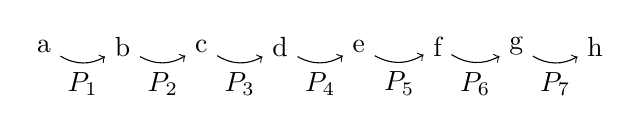
\begin{tikzpicture}
		\node (A) at (0,0) {a};
		\node (B) at (1,0) {b};
		\node (C) at (2,0) {c};
		\node (D) at (3,0) {d};
		\node (E) at (4,0) {e};
		\node (F) at (5,0) {f};
		\node (G) at (6,0) {g};
		\node (H) at (7,0) {h};
		
		\draw[->, bend right] (A) to node[midway, below] {$P_1$} (B);
		\draw[->, bend right] (B) to node[midway, below] {$P_2$} (C);
		\draw[->, bend right] (C) to node[midway, below] {$P_3$} (D);
		\draw[->, bend right] (D) to node[midway, below] {$P_4$} (E);
		\draw[->, bend right] (E) to node[midway, below] {$P_5$} (F);
		\draw[->, bend right] (F) to node[midway, below] {$P_6$} (G);
		\draw[->, bend right] (G) to node[midway, below] {$P_7$} (H);
	\end{tikzpicture}
	
	\nn
	
	Step $j=1$
	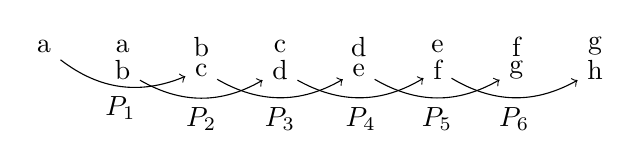
\begin{tikzpicture}
		\node (A2) at (-1,0) {a};
		\node (A) at (0,0) {a};
		\node (B) at (1,0) {b};
		\node (B2) at (0,-0.3) {b};
		\node (C) at (2,0) {c};
		\node (C2) at (1,-0.3) {c};
		\node (D) at (3,0) {d};
		\node (D2) at (2,-0.3) {d};
		\node (E) at (4,0) {e};
		\node (E2) at (3,-0.3) {e};
		\node (F) at (5,0) {f};
		\node (F2) at (4,-0.3) {f};
		\node (G) at (6,0) {g};
		\node (G2) at (5,-0.3) {g};
		\node (H2) at (6,-0.3) {h};
		
		\draw[->, bend right] (A2) to node[midway, below] {$P_1$} (C2);
		\draw[->, bend right] (B2) to node[midway, below] {$P_2$} (D2);
		\draw[->, bend right] (C2) to node[midway, below] {$P_3$} (E2);
		\draw[->, bend right] (D2) to node[midway, below] {$P_4$} (F2);
		\draw[->, bend right] (E2) to node[midway, below] {$P_5$} (G2);
		\draw[->, bend right] (F2) to node[midway, below] {$P_6$} (H2);
	\end{tikzpicture}
	
	Step $j=2$
	\begin{tikzpicture}
		\node (A3) at (-1,0) {a};
		
		\node (A) at (0,0) {a};
		\node (A) at (1,0) {a};
		\node (A) at (2,0) {a};
		
		\node (B3) at (0,-0.3) {b};
		
		\node (B) at (1,-0.3) {b};
		\node (B) at (2,-0.3) {b};
		\node (B) at (3,0) {b};
		
		\node (C3) at (1,-0.6) {c};
		
		\node (C) at (2,-0.6) {c};
		\node (C) at (3,-0.3) {c};
		\node (C) at (4,0) {c};
		
		\node (D3) at (2,-0.9) {d};
		
		\node (D) at (3,-0.6) {d};
		\node (D) at (4,-0.3) {d};
		\node (D) at (5,0) {d};
		
		\node (E3) at (3,-0.9) {e};
		
		\node (E) at (4,-0.6) {e};
		\node (E) at (5,-0.3) {e};
		\node (E) at (6,0) {e};
		
		\node (F3) at (4,-0.9) {f};
		
		\node (F) at (5,-0.6) {f};
		\node (F) at (6,-0.3) {f};
		
		\node (G3) at (5,-0.9) {g};
		
		\node (G) at (6,-0.6) {g};
		
		\node (H3) at (6,-0.9) {h};
		
		\draw[->, bend right] (A3) to node[midway, below] {$P_1$} (E3);
		\draw[->, bend right] (B2) to node[midway, below] {$P_2$} (F3);
		\draw[->, bend right] (C3) to node[midway, below] {$P_3$} (G3);
		\draw[->, bend right] (D3) to node[midway, below] {$P_4$} (H3);
	\end{tikzpicture}
\end{center}

Facendo tutte le somme in quest'ordine, ogni cella \textbf{conterrà la somma delle precedenti}, l'algoritmo \textbf{termina} una volta arrivati al punto in cui \textbf{nessun elemento ha un successore} in range, ovvero il "salto" di celle porta tutti gli elementi fuori range.\\

\newpage

%\paragraph{Valutazione:} 
Quanti passi sono necessari? Si completa quando nessun elemento ha un successore, considerando che al $j$-esimo passo sono presenti $2^j$ elementi senza successori, l'ultimo passo dell'algoritmo è quando $2^j = n \implies j = \log n$, \textbf{servono} $\log n$ \textbf{passi}.\\

Ad ogni passaggio vengono \textbf{usati $n-2^j$ processori}, quindi vengono usati tutti i processori con indice $1 \leq k \leq n - 2^{j-1}$.\\

Poniamo nel vettore $S[k]$ la posizione del \textbf{successore} di $M[k]$ (la cella legata), come viene \textbf{inizializzato} prima dell'esecuzione dell'algoritmo vero e proprio?
$$S[k] = k+1 \; \text{ e } \; S[n] = 0$$
Con $n$ indice dell'ultima cella (dimensione del problema).\\

Dato il processore $P_k$, quale istruzione su $M$ deve eseguire? 
$$ M[S[k]] \leftarrow M[k] + M[S[k]] $$

Poi bisogna aggiornare $S$:
$$ S[k] \leftarrow \left(S[k] == 0? 0 : S[S[k]] \right) $$
Se $S[k] = 0$ rimane $0$, altrimenti diventa $S[S[k]]$.\\

Codice dell'algoritmo parallelo (con $M$ ed $S$ già inizializzati):
\begin{lstlisting}[escapeinside={(*}{*)}]
	for (*$j=1$*) to (*$\log n$*) do 
		for (*$1 \leq k \leq n-2^{j-1}$*) par do
			M[S[(*$k$*)]] = M[(*$k$*)] + M[S[(*$k$*)]]
			S[(*$k$*)]  = (S[(*$k$*)]==0) ? 0 : S[S[(*$k$*)]]
\end{lstlisting}

All'inizio l'unico elemento che non ha successore, ovvero con $S[k] = 0$ è l'ultimo, ad ogni passo parallelo se ne aggiungono $2^{j-1}$ (si arriva a $2^j$).\\

\newpage

\paragraph{Questo algoritmo è EREW?} La \textbf{scrittura è esclusiva} ma ogni processore deve \textbf{leggere} anche da una \textbf{cella che verrà usata anche dai processori adiacenti}, però \textbf{ognuno} di questi lo farà in \textbf{tempi diversi}: $k$ accederà prima alla cella $M[k]$ poi a $M[S[k]]$, mentre $k+1$ accederà ad $M[S[k]]$ e poi ad $M[S[S[k]]]$. Questi sono passi paralleli quindi \textbf{la stessa cella non verrà usata nello stesso momento}.\\
L'algoritmo \textbf{è EREW}.\\

%Guarda slide? Aggiungi qualcosa? Ma cazzo ne so

\paragraph{Correttezza:}
\begin{enumerate}
	\item è \textbf{EREW PRAM}: $P_k$ lavora su $M[k]$ e $M[S[k]]$: se $i \neq j \implies S[i] \neq S[j]$, quindi hanno successori diversi (se non sono 0)
	\item \textbf{dimostro} $M[k] = \sum_{i=1}^k M[i]$, $1 \leq k \leq n$. Si lavora sulla proprietà del $j$-esimo passo:
	$$ M[k] = \begin{cases}
		M[k] + \, ... \, + M[1] & k \leq 2^j \\
		M[k] + \, ... \, + M[t- 2^j + 1] & k > 2^j
	\end{cases}
	$$
	C'è sempre la somma dei $2^j$ elementi precedenti, sia che si arrivi a $1$ che a $t-2^j+1$. \\
	Se questa proprietà è vera si ha per $j=\log n$ (ultimo passo):
	$$ M[k] = \begin{cases}
		M[k] + \, ... \, + M[1] & k \leq 2^j = 2^{\log n} = n \\
		... & k>2^j = n
	\end{cases}
	$$
	
	Si dimostra per induzione su $j$:
	\begin{itemize}
		\item \textbf{Base}: $j=1$, per $k \leq 2$
		$$ 
		\begin{array}{c c}
			k = 1 & M[1] \leftarrow M[1]  \\
			k = 2 & M[2] \leftarrow M[1] + M[2]
		\end{array}
		$$
		per $k > 2$:
		$$ 
		M[t + 1] \leftarrow M[t] + M[t+1] = M[k-1] + M[k] \rightarrow M[k]
		$$
		Quindi il caso base è vero.\\
		
		%End L8, classe
		
		\newpage
		
		\item \textbf{Passo induttivo}: si presuppone vera la proprietà per il passo $j-1$ e bisogna dimostrare che vale per $j$. \\
		Prima di iniziare il $j$-esimo passo quanto vale $S$?
		$$ S[k] = \begin{cases}
			k + 2^{j-1} & k \leq n-2^{j-1} \\
			0 & k > n - 2^{j-1}
		\end{cases}$$
		I legami al $j$-esimo passo legano numeri a distanza $2^{j-1}$.\\
		Le celle con indice $\leq 2^{j-1}$ sono già a posto, in quanto la proprietà è vera per $j-1$.\\
		
		Le celle con indice compreso tra $2^{j-1}$ e $2^j$, hanno indice $t$ indicato come:
		$$ 2^{j-1} \leq t \leq 2^j \implies t = 2^{j-1} + a$$
		
		Quindi sappiamo che 
		$$ M[a + 2^{j-1}] \leftarrow M [a] + M[a + 2^{j-1}]$$
		
		Ma $a$ è per forza $\leq 2^{j-1}$ e $t$ invece è $t > 2^{j-1}$, quindi, per ipotesi induttiva, i valori di $M [a]$ e $M[a + 2^{j-1}]$ corrispondono a:
		$$ M[1] + \, ...\, + M[a] \; + \; M[a+1] + \, ... \, + M[a+2^{j-1}] $$
		
		Invece, per le celle con indice $t > 2^j$, quindi $t = 2^j + a$. Gli elementi sommati in $M[a + 2^j]$ sono: 
		$$ M[a + 2^j] \leftarrow M[a + 2^{j-1}] + M[a + 2^j] $$
		
		Ma, considerando che l'indice è $> 2^{j-1}$, per ipotesi induttiva, corrispondono a:
		$$ M[a + 1] + \, ... \, + M[a + 2^{j-1}] \; + \; M[a + 2^{j-1} + 1] + \, ... \, + M[a + 2^j] $$
		
		E di conseguenza la proprietà continua a essere vera.
	\end{itemize}
\end{enumerate}

% End L8 videolez

\newpage

\paragraph{Valutazione dell'algoritmo:} Il \textbf{numero di processori} massimo è 1 in meno rispetto alla dimensione dell'input, usati nel primo passo:
$$ p(n) = n-1 $$

Per quanto riguarda il \textbf{tempo}, si ha un ciclo \texttt{for} con $\log n$ passi, con all'interno un \texttt{par do} che fa eseguire in parallelo ai processori 2 istruzioni, somma e aggiornamento del vettore $S$.\\
La prima istruzione
$$ M[S[k]] = M[k] + M[S[k]] $$
è composta da 5 microistruzioni
\begin{center}
	\begin{tabular}{c c}
		\texttt{LOAD} & $M[k]$ \\
		\texttt{LOAD} & $S[k]$ \\
		\texttt{LOAD} & $M[S[k]]$ \\
		\texttt{ADD} & \\
		\texttt{STORE} & $M[S[k]]$ \\
	\end{tabular}
\end{center}
Mentre l'istruzione di aggiornamento
$$ S[k] = (S[k]==0 ? 0 : S[S[k]]) $$
è composta da 4 microistruzioni
\begin{center}
	\begin{tabular}{c c}
		\texttt{LOAD} & $S[k]$ \\
		\texttt{JZERO} & \\
		\texttt{LOAD} & $S[S[k]]$ \\
		\texttt{STORE} & $S[k]$
	\end{tabular}
\end{center}

Quindi in totale sono $9$ operazioni svolte $\log n$ volte, ottenendo un \textbf{tempo}: 
$$ T(n,n-1) \sim 9 \log n $$

Di conseguenza l'\textbf{efficienza} è:
$$ E(n, p(n)) = \frac{n-1}{(n-1) 9 \log n} = \frac{1}{9 \log n} \rightarrow 0 \; \text{ (lentamente)} $$

\newpage

Sfruttando \textbf{Wyllie}, come per la sommatoria, in modo da far \textbf{tendere l'efficienza} a \textbf{una costante} (far sparire la funzione $\log n$ da $E$).\\

Vogliamo migliorare l'uso dei processori, raggruppiamo di $\log n$ in $\log n$ i valori da sommare, con un processore che esegue somme in sequenza per ognuno. Di conseguenza: 
$$ p(n) = o \left(\frac{n}{\log n}\right), \;\; T(n, p(n)) = O (\log n) \;\; E \rightarrow C \neq 0 $$

Il primo passo è sequenziale su $\log n$ numeri, ogni processore effettua la somma sequenziale di $\log n$ numeri, di conseguenza il numero di processori passa da lineare a $n/\log n$. Il tempo rimane logaritmico per la fase parallela, ma si aggiunge tempo logaritmico per la fase sequenziale $\sim O (\log n)$. Nel calcolo dell'efficienza $\log n$ adesso si semplifica e rimane che tende a una costante $\neq 0$.\\

Come per la sommatoria, anche l'\textbf{algoritmo} per le somme prefisse può essere \textbf{usato per un problema generale} "op-prefissa", con operazione associativa:
\begin{itemize}
	\item Input: $M[1], \, ... \, , M[n]$, $n$ celle
	\item Output: $M[k] = OP_{i = 1}^k M[i]$, $1 \leq k \leq n$, in ogni cella ci sia il risultato dell'operazione sulle $k$ celle precedenti 
\end{itemize}

L'operazione deve essere associativa come ad esempio: $+, *, \wedge, \vee, \min, \max, \, ...$.\\

\newpage

\subsection{Valutazione di polinomi}
Si tratta di un problema che prende in input un polinomio $p(x)$ di grado $n$ e un valore $\alpha$, restituendo il polinomio valutato sul valore $\alpha$, quindi $p(\alpha)$.\\

\textbf{Definizione}:
\begin{itemize}
	\item \textbf{Input:} $p(x) = a_0 + a_1 x + a_2 x^2 + \, ... \, + a_n x^n$, $\alpha$
	\item \textbf{Output:} $p(\alpha)$
\end{itemize}

Dati \textbf{in memoria}: 
\begin{itemize}
	\item il \textbf{valore} $\alpha$
	\item $a_0, a_1, \, ... \, , a_n \rightarrow A[0], A[1], \, ... \, A[n]$, $n$ celle nella memoria condivisa, da $A[0]$ ad $A[n]$, per \textbf{contenere} i \textbf{coefficienti}
\end{itemize}

Algoritmo sequenziale tradizionale:
\begin{itemize}
	\item prodotti: $\sum_{i=0}^n i \sim n^2$
	\item somme: $n$
\end{itemize}
Di conseguenza, in totale $\sim n^2$.\\

Ma si può fare di meglio, \textbf{miglioramento di Ruffini-Horner}: l'idea è raccogliere $x$ in maniera iterata:
$$ \begin{array}{c c c}
	p(n) & = & a_0 + a_1 x + a_2 x^2 + a_3 x^3 + a_4 x^4 \\
	& = & a_0 + x (a_1 + a_2 x + a_3 x^2 + a_4 x^3) \\ 
	& = & a_0 + x (a_1 + x (a_2 + a_3 x + a_4 x^2)) \\
	& = & a_0 + x (a_1 + x (a_2 + x (a_3 + a_4 x))) \\
\end{array}$$

\textbf{Generalizzando}:
$$ p(x) = a_0 x(a_1 + \, ... \; a_{n-2} + x (a_{n-1} + a_n x) \, ... \,)$$

Questa forma del polinomio suggerisce un algoritmo, \textbf{sostituendo} $\alpha$ a \textbf{partire} dall'\textbf{ultimo coefficiente} del polinomio, partendo dalla parentesi più interna (e chiamo questo valore ottenuto $p$). Quindi, sostituisco $\alpha$, sommo un coefficiente e ripeto fino ad arrivare alla fine
$$ p = a_n \cdot \alpha + a_{n-1} \rightarrow p = a_{n-2} + p \cdot \alpha \rightarrow  \; ...$$
Quindi: 
$$ p = a_j + p \cdot \alpha $$

\newpage

Codice per l'algoritmo sequenziale Ruffini-Horner:
\begin{lstlisting}[escapeinside={(*}{*)}]
	Input ((*$\alpha$*))
	p = (*$a_n$*)
	for (*$i=1$*) to (*$n$*)
		p = (*$a_{n-i}$*) + p(*$\cdot \alpha$*)
	Output(p)
\end{lstlisting}

Prestazioni sequenziali: 2 operazioni per il numero di iterazioni
$$ T(n, 1) = 2n $$
Lineare, meglio che $n^2$ di prima.\\

Possibile \textbf{algoritmo parallelo}:
\begin{itemize}
	\item \textbf{Costruisco} il \textbf{vettore} delle \textbf{potenze di} $\alpha$: $Q$
	$$ Q[k] = \alpha^k \;\;\; 0 \leq k \leq n $$
	Memorizzo le potenze di $\alpha$ nel vettore $Q$. \\
	
	\item Eseguo il \textbf{prodotto interno} $<A,Q>$
	$$ <A, Q> = \sum_{k=0}^n A[k] \cdot Q[k] $$
	dive $A$ è il vettore dei coefficienti. Questo effettivamente è valutare il polinomio su $\alpha$. \\
	
	\item \textbf{Restituisco} $<A, Q>$. \\
\end{itemize}

Il prodotto interno parallelo lo abbiamo già visto ed è efficiente, rimane da capire se è parallelizzabile efficientemente la creazione del vettore $Q$.\\

\newpage

Per \textbf{creare} $Q$:
\begin{itemize}
	\item \textbf{Pongo} $\alpha$ in \textbf{tutti gli elementi di} $Q$ da 1 a $n$
	$$ Q[1] = \alpha, Q[2] = \alpha, \, ... \, , Q[n] = \alpha $$
	Non si considera la cella $Q[0]$, che deve contenere 1. Questo è un problema di replica.\\
	
	\item Applico il \textbf{prodotto-prefisso su} $Q$: 
	$$ Q[1]= \alpha, Q[2] = \alpha^2 , \, ... \, , Q[n] = \alpha^n $$
\end{itemize}

% End videolez 9


\paragraph{Come risolvere replica in parallelo:} prima idea, algoritmo CREW, $n$ processori copiano nelle $n$ celle il valore $\alpha$
\begin{lstlisting}[escapeinside={(*}{*)}]
	for (*$k = 1$*) to (*$n$*) par do
		Q[(*$k$*)] = (*$\alpha$*)
\end{lstlisting}
\textbf{Prestazioni}: 
$$ p = n, \;\; t = 2, \;\; E \sim \frac{n}{n \cdot 2} \rightarrow c \neq 0 $$

\nn

Seconda idea, per \textbf{abbassare} il \textbf{numero di processori} usati dalla replica: \textbf{Wyllie}, raggruppo gli $n$ processori in $\log n$ elementi, quindi il processore $k$ si occuperà di caricare $\alpha$ nelle celle di posizione tra $(k-1) \log n + 1$ e $k \log n$.\\

Codice: 
\begin{lstlisting}[escapeinside={(*}{*)}]
	for (*$k = 1$*) to (*$\sfrac{n}{\log n}$*) par do 
		for (*$i = 1$*) to (*$\log n$*) do
			Q[(*$(k-1) \log n + i$*)] = (*$\alpha$*)
\end{lstlisting}
Il numero di processori è di $n/\log n$, di conseguenza le \textbf{prestazioni}: 
$$ p = \frac{n}{\log n}, \;\; t = c \log n, \;\; E = \frac{n}{\frac{n}{\log n} \cdot c \log n}  = \frac{1}{c} \neq 0 $$
Comunque si tratta di un algoritmo CREW.\\

\newpage

Problema: tutti leggono $\alpha$ contemporaneamente, rendendo l'algoritmo CREW, quindi, terza idea, \textbf{per renderlo EREW-PRAM}: 
\begin{itemize}
	\item \textbf{Costruisco} il \textbf{vettore} $\alpha, 0, 0, \, ... \, , 0$
	\item Eseguo \textbf{somme-prefisse}
\end{itemize}

Codice per \textbf{ottenere il vettore} $\alpha, 0, 0, \, ... \, , 0$
\begin{lstlisting}[escapeinside={(*}{*)}]
	Input ((*$\alpha$*))
	Q[1] = (*$\alpha$*)
	for (*$k = 2$*) to (*$n$*) par do
		Q[(*$k$*)] = 0 
\end{lstlisting}
Lo 0 è una costante e non deve essere letta.\\

Riduzione dei processori: richiederà numero di processori $p = n/\log n$ e $t = \log n$ ad entrambi gli step, quindi in totale
$$ p = \frac{n}{\log n}, \;\; t = \log n, \;\; E = c \neq 0 $$

\paragraph{Riassunto:} valutazione polinomio con EREW-PRAM:
\begin{itemize}
	\item Costruisco $Q[k] = \alpha$ con replica
	$$ p = \frac{n}{\log n}, \;\; t = \log n $$
	
	\item Costruisco $Q[k] = \alpha^k$ con prodotto prefisso
	$$ p = \frac{n}{\log n}, \;\; t = \log n $$
	
	\item Calcolo il prodotto interno $\langle A, Q \rangle$
	$$ p = \frac{n}{\log n}, \;\; t = \log n $$
\end{itemize}
In totale:
$$ p = \frac{n}{\log n}, \;\; t = \log n, \;\; E = \frac{T(n,1)}{p(n) T(n, p(n))} \sim \frac{2n}{\frac{n}{\log n} \log n} \rightarrow c \neq 0 $$

\newpage

%Nuovo problema

\subsection{Ricerca di un elemento}
Trovare se il valore $\alpha$ è presente tra le $n$ celle, l'ultima cella assumerà valore $1$ se esiste il valore cercato all'interno della memoria considerata. Definizione: 
\begin{itemize}
	\item \textbf{Input:} $M[1], M[2], \, ... \, , M[n]$, $\alpha$
	\item \textbf{Output:} $M[n] = 1$ se $\exists k$ t.c. $M[k] =\alpha$, altrimenti $0$
\end{itemize}

Algoritmo sequenziale classico: $t=n$ controllo tutte le celle; se il vettore è ordinato (ordinamento costo $O(n \log n)$) posso fare ricerca dicotomica ($t = \log n$).\\
Algoritmo quantistico (recente, del 1996) su input non ordinato (interferenza quantistica): $t = \sqrt{n}$.\\

Algoritmi \textbf{paralleli per ricerca} di $\alpha$: prima idea, CRCW, si usa un flag $F$
\begin{lstlisting}[escapeinside={(*}{*)}]
	F = 0
	for (*$k=1$*) to (*$n$*) par do
		if (M[(*$k$*)] == (*$\alpha$*))
			F = 1
	M[(*$n$*)] = F
\end{lstlisting}

Se uno degli $n$ processori trova nella sua cella dedicata il valore corretto il flag viene messo ad uno, il valore del flag viene messo in $M[n]$ alla fine. Abbiamo una lettura concorrente di $\alpha$ ed una scrittura concorrente di $F$ per tutti i processori che trovano $\alpha$ nello stesso momento.\\

Prestazioni: 
$$ p(n) = n \;\;\;\;\; t = c $$

Perché usiamo $F$? Per non perdere il valore di $M[n]$?

\newpage

\textbf{Seconda idea}: algoritmo CREW
\begin{lstlisting}[escapeinside={(*}{*)}]
	for (*$k=1$*) to (*$n$*) par do 
		M[(*$k$*)] = (M[(*$k$*)] == (*$\alpha$*) ? 1 : 0)
	
	Max-Iterato(M[1], ... , M[(*$n$*)])
\end{lstlisting}

Il risultato viene scritto in ogni cella, e poi bisogna mettere $1$ in $M[n]$ se c'è almeno un $1$ all'interno delle celle. Per l'ultimo passaggio si può fare un Max-Iterato su tutte le celle (stesso modulo della somma-iterata).\\

\textbf{Prestazioni}: 
\begin{itemize}
	\item Per la prima parte: $p(n) = n, \;\; t = c$, ma applicando Wyllie: 
	$$ \implies p(n) = \frac{n}{\log n} \;\;\;\; t = \log n$$
	\item Per il Max-Iterato 
	$$ p(n) = \frac{n}{\log n} \;\;\;\; t = \log n $$
\end{itemize}
Risultato: 
$$ p(n) = O (n/\log n) \;\;\;\; t = O (\log n) $$
L'efficienza: 
$$ E \rightarrow c \neq 0$$

\newpage

\textbf{Terza idea}: algoritmo EREW
\begin{enumerate}
	\item Usa modulo replica per $\alpha$
	$$ \alpha \rightarrow A[1], \, ... \, , A[n] $$
	\item Confronto con tutte le celle: 
	\begin{lstlisting}[escapeinside={(*}{*)}]
	for (*$k=1$*) to (*$n$*) par do 
		M[(*$k$*)] = (M[(*$k$*)] == A[(*$k$*)] ? 1 : 0)
	\end{lstlisting}
	\item Max-iterato($M[1], \, ... \, , M[n]$) per spostare il valore $1$ nell'ultima cella
\end{enumerate}

\textbf{Prestazioni}: 
Step 2 e 3 vengono risolti (come nel precedente) con $ p(n) = n/\log n$ e $t = \log n$.  Mentre il passo 1 $ p(n) = n/\log n$ e $t = \log n$.\\
Totale: 
$$ p = \frac{n}{\log n}, \;\; t = \log n, \;\; E = c \neq 0 $$

Quindi abbiamo un algoritmo parallelo EREW efficiente.\\

\vfill

\paragraph{Varianti di questo codice per problemi legati:}
\begin{itemize}
	\item \textbf{conteggio di} $\alpha$ \textbf{in} $M$: il Max-Iterato diventa una sommatoria, conta quante celle hanno trovato il valore
	\item \textbf{posizione massima di} $\alpha$ \textbf{in} $M$: al posto di scrivere $1$ se trovo il valore scrivo $k$, dove questo è l'indice della cella 
	\item \textbf{posizione minima di} $\alpha$ \textbf{in} $M$: modifico come sopra scrivendo $k$ al posto che $1$ ma l'ultimo passaggio diventa una OP-Iterata, dove
	$$ OP (x,y) = \begin{cases}
		\min (x,y) & \text{ if } x \neq 0 \text{ and } y \neq 0 \\
		\max (x,y) & \text{ otherwise}
	\end{cases}$$
\end{itemize}


\newpage

\subsection{Problema dell'ordinamento}

Formalmente chiamato \textbf{ranking}. Definizione:
\begin{itemize}
	\item \textbf{Input:} $M[1], \, ... \, , M[n]$
	
	\item \textbf{Output:} permutazione $p: \{1, \, ... \, , n\} \rightarrow \{1, \, ... \, , n\}$ tale che
	$$ M[p(1)] \leq M[p(2)] \leq \, ... \, \leq M[p(n)] $$
	dove $p(i)$ indica l'indice dell'elemento del vettore $M$ in che va in posizione $i$
\end{itemize}

In genere gli algoritmi di ordinamento sono basati sui confronti, guardano chi è il più piccolo.\\
Gli algoritmi di ordinamento basati sul confronto hanno 
$$ t = \Theta (n \log n) $$

Dimostrazione (circa) del \textbf{lower bound}: albero di decisione = algoritmo di ordinamento. Costruisco un albero in cui ad ogni nodo avviene un confronto.\\
Esempio di nodo: 
\begin{center}
	\begin{tikzpicture}
		\node (A) at (0,0) {$a \leq b$};
		\node (B) at (-2,-2) {$b \leq c$};
		\node (C) at (2,-2) {$d \leq e$};
		
		\draw[->] (A) to node[midway, above] { sì } (B);
		\draw[->] (A) to node[midway, above] { no } (C);
	\end{tikzpicture}
\end{center}

Le foglie sono una permutazione che permette di ordinare l'input.\\
L'altezza dell'albero rappresenta il numero di confronti effettuati nel caso peggiore, di conseguenza il tempo dell'algoritmo di ordinamento.\\

\textbf{Osservazione}: il numero di foglie deve essere $\geq n!$ in quanto questi sono i possibili ordinamenti di $n$ elementi.\\
Per un albero di altezza $t$ il numero massimo di foglie è $2^t$
$$ 2^t \geq \text{ foglie } \geq n! \implies t \geq \log n! $$
$$ \log n! \geq \log \prod_{i = n/2 + 1}^n i \geq \log \left(\frac{n}{2}\right)^{n/2} = \frac{n}{2} \log \frac{n}{2} \sim n \log n $$

\newpage

\subsubsection{CountingSort}

\textbf{Primo approccio parallelo } (basato su algoritmo di conteggio $t = \Theta (n^2)$).\\

Assunzione: $n$ è una potenza di 2 e gli elementi sono $\neq$ tra loro.\\

Sequenziale CountingSort: $M[i]$ va in posizione $k$ $\Leftrightarrow$ $k$ elementi sono $\leq M[i]$ in $M$.\\

Usiamo il vettore 
$$ V[1], V[2], \, ... \, , V[n] \; \text{ dove }\; V[i] = k $$

Algoritmo sequenziale counting:
\begin{lstlisting}[escapeinside={(*}{*)}]
	for (*$i = 1$*) to (*$n$*)
		V[(*$i$*)] = 0
	
	for (*$i=1$*) to (*$n$*)
		for (*$j=1$*) to (*$n$*)
			if (M[(*$j$*)] < M[(*$i$*)])
				V[(*$i$*)]++
	
	for (*$i=1$*) to (*$n$*)
		F[V[(*$i$*)]] = M[(*$i$*)]
	for (*$i=1$*) to (*$n$*)
		M[(*$i$*)] = F[(*$i$*)]
\end{lstlisting}

Conto quante celle hanno valore minore di $M[i]$ ed ottengo la posizione del valore nel vettore finale.\\
Gli ultimi due \texttt{for} servono a riscrivere il vettore in modo ordinato.\\

%Slide 10 su 12
%End lezione 10

\paragraph{Prestazioni:} la fase pesante è quella dei 2 \texttt{for} innestati, effettua $n^2$ confronti, quindi $T(n,1) = n^2$.\\

\newpage

\paragraph{Versione parallela:} passaggi

\begin{enumerate}
	\item $\forall j,i$ ho un \textbf{processore} $P_{i,j}$ che effettua 
	$$ M[j] \leq M[i] ? $$
	Poniamo il \textbf{risultato} del confronto in una \textbf{matrice booleana}
	$$ V[i,j] = (M[j] \leq M[i] ? 1 : 0 )$$
	Quindi la $i$-esima riga individua gli elementi di $M$ che sono $\leq M[i]$.\\
	
	\item $\forall i$ effettuo la \textbf{sommatoria parallela} della $i$-esima riga (sommo i valori interni a tutta la riga, ogni riga), ottenendo
	$$
	\implies \begin{array}{c}
		V[1,n] \\
		V[2,n] \\
		\vdots \\
		V[n,n] \\
	\end{array}
	\xrightarrow[\text{ (di prima) }]{\text{ coincide con }}
	\begin{array}{c}
		V[1] \\
		V[2] \\
		\vdots \\
		V[n] \\
	\end{array}
	$$
	In questo modo, alla fine della somma, trovo quanti valori sono inferiori di $i$.\\
\end{enumerate}

\paragraph{Codice:} 
\begin{lstlisting}[escapeinside={(*}{*)}]
	for (*$1 \leq i$*), (*$j \leq n$*) par do
		V[(*$i$*), (*$j$*)] = (M[(*$j$*)] (*$\leq$*) M[(*$i$*)] ? 1 : 0)
	for (*$i=1$*) to (*$n$*) par do
		Sommatoria(V[(*$i,1$*)], V[(*$i,2$*)], ... , V[(*$i,n$*)])
	for (*$i=1$*) to (*$n$*) pardo
		M[V[(*$i$*), (*$n$*)]] = M[(*$i$*)]
\end{lstlisting}

Per \textbf{ogni coppia} $i,j$ c'è \textbf{un processore} che lavora in parallelo per eseguire il confronto, il \textbf{risultato} viene \textbf{memorizzato} nella cella $V[i,j]$ di una \textbf{matrice booleana}. Vuol dire che ci sono $n^2$ \textbf{processori}.\\
Poi viene effettuata la \textbf{somma parallela} dei valori presenti in \textbf{ogni riga}.\\
Infine si va a \textbf{scrivere} nel vettore $M$ \textbf{l'array ordinato}. Ogni valore $V[i,n]$ va ad indicare quanti elementi sono minori di $i$.\\

\paragraph{Prestazioni:} si tratta di un algoritmo CREW (accesso concorrente nella prima fase)
\begin{itemize}
	\item Prima fase: 
	$$ p(n) = n^2, \;\;\;\; T(n, n^2) = 4 $$
	Per il tempo le fasi sono \texttt{LD}, \texttt{LD}, \texttt{JZ}, \texttt{ST}. Usando Wyllie si può ottenere
	$$ p(n) = n^2/\log n, \;\;\;\; t \sim \log n $$
	
	\item Seconda fase: $n$ moduli sommatoria, quindi 
	$$ p(n) = n^2/\log n, \;\;\;\; t \sim \log n $$
	
	\item Terza fase 
	$$ p(n) = n \;\;\;\; t = 3 $$
\end{itemize}

In \textbf{totale}
$$ p \sim \frac{n^2}{\log n}, \;\;\;\; t \sim \log n $$
$$ E = \frac{n \log n}{\frac{n^2}{\log n} \cdot \log n}  = \frac{\log n}{n} \rightarrow 0 $$
Quindi non è efficiente.\\

\vfill

\paragraph{Algoritmi di ordinamento paralleli: }
\begin{itemize}
	\item \textbf{CountingSort}: 
	$$ E =  \frac{\log n}{n} \rightarrow 0 $$
	\item \textbf{BitSort}:
	$$ E = \frac{1}{\log n} \rightarrow 0 $$
	ma ci tende lentamente
	\item \textbf{Cole} (1988)
	$$ E \rightarrow c \neq 0 $$
	ma è complicato
\end{itemize}

\newpage

\subsubsection{BitSort}

Algoritmo sequenziale MergeSort: dai che sai come funziona, non devo scrivertelo. Tempo: $T(n, 1) = n \log n$.\\

Prendendo ispirazione dal MergeSort, effettuarlo in parallelo vorrebbe dire effettuare $\log n$ passi paralleli.\\

Ma purtroppo \textbf{NON è parallelizzabile} ed ottengo angora $t \sim n \log n$.\\

\textit{Quando il passaggio di merge dei valori diventa facile?} Quando i \textbf{due vettori} sono \textbf{ordinati} ed i \textbf{valori del primo} sono \textbf{tutti minori} dei \textbf{valori del secondo}, in questo caso per effettuare il merge è sufficiente concatenare i due vettori.\\

Con l'uso di sequenze di numeri bitoniche possiamo garantire che questa proprietà sia rispettata.\\

\paragraph{Operazioni elementari su sequenze: }
\begin{itemize}
	\item \textbf{Reverse}: inverte il vettore
	$$ REV(A[1], A[2], \, \dots \, , A[n]) $$
	$$ A[1] \leftarrow A[n], \;\; A[2] \leftarrow A[n-1], \;\; \dots \;\; A[n] \leftarrow A[1] $$
	
	\item \textbf{MinMax}: divide il vettore in due, prende l'elemento $k$ e l'elemento $k + n/2$, rispettivamente per la prima e seconda metà. Nel primo dei due scrive il minimo dei due, nel secondo scrive il massimo. Ripeto l'operazione per tutti gli elementi delle metà. In questo modo nella prima metà avrò tutti i minimi, nella seconda tutti i massimi. 
	$$ A[1] \, \dots \, A[k], \, \dots \, A[\sfrac{n}{2}] \, \dots \, A[k + \sfrac{n}{2}] \, \dots \, A[n]$$
	$$ A[k] \leftarrow \min \{A[k], A[k + \sfrac{n}{2}]\}, \;\; A[k + \sfrac{n}{2}] \leftarrow \max \{A[k], A[k + \sfrac{n}{2}]\}, \;\; \dots $$
\end{itemize}

\newpage


\paragraph{Algoritmi paralleli per queste operazioni: }
\begin{itemize}
	\item \textbf{Procedura} $Rev(A)$: da 1 a $n/2$, scambio i valori di ogni cella con la sua simmetrica
	\begin{lstlisting}[escapeinside={(*}{*)}]
	for (*$1 \leq k \leq \sfrac{n}{2}$*) par do
		Swap(A[(*$k$*)], A[(*$n-k+1$*)])
	\end{lstlisting}
	Prestazioni: lavora su metà dei valori e deve fare \texttt{LD}, \texttt{LD}, \texttt{ST}, \texttt{ST}
	$$ p(n) = \frac{n}{2}, \;\;\;\; t = 4 $$
	
	\item \textbf{Procedura} $MinMax(A)$:
	\begin{lstlisting}[escapeinside={(*}{*)}]
	for (*$1 \leq k \leq \sfrac{n}{2}$*) par do
		if (A[(*$k$*)] > A[(*$k + \sfrac{n}{2}$*)])
			Swap(A[(*$k$*)], A[(*$k + \sfrac{n}{2}$*)])
	\end{lstlisting}
	Prestazioni: richiede solamente un'operazione in più di prima (il confronto)
	$$ p(n) = \frac{n}{2}, \;\;\;\; t = 5 $$
\end{itemize}

\paragraph{Particolari sequenze numeriche:} Definizioni formali: 
\begin{itemize}
	\item \textbf{Unimodale}: $A$ è unimodale iff $\exists k$ tale che 
	$$ A[1] > A[2] > \, \dots \, > A[k] < A[k+1] < \, \dots \, < A[n] $$
	oppure 
	$$ A[1] < A[2] < \, \dots \, < A[k] > A[k+1] > \, \dots \, > A[n] $$
	
	\item \textbf{Bitonica}: $A$ è bitonica iff $\exists$ una permutazione ciclica di $A$ tale che dia una sequenza unimodale: $\exists j$ tale che
	$$ A[j], \, \dots \, , A[n], A[1], \, \dots \, , A[j-1] $$ 
	è unimodale
\end{itemize}
Sostanzialmente, una sequenza unimodale ha un picco (massimo o minimo), mentre una bitonica ha due picchi , un minimo ed un massimo (scende, sale e poi scende di nuovo o viceversa) e se la "giro" può diventare un picco solo. \\
%Da mettere sotto? Da fare grafico? Chi lo sa

\newpage

\textbf{Esempi}: 
$$ 2 \;\; 4 \;\; 7 \;\; 9 \;\; 5 \;\; 3 $$
è una serie unimodale, con $9$ come picco.\\

$$ 7 \;\; 9 \;\; 5 \;\; 3 \;\; 2 \;\; 4 $$
è una serie bitonica, con $9$ e $2$ come picchi (sale, poi scende, poi risale) e posso "girarla" fino a farla diventare quella di prima.\\

%Slide 12/14
%End L11

\paragraph{Osservazioni: }
\begin{itemize}
	\item \textbf{Unimodale} $\implies$ \textbf{bitonica}, grazie alla permutazione identità.\\
	
	\item In una serie \textbf{bitonica}, gli \textbf{elementi di fine array} devono essere \textbf{maggiori} di quelli di \textbf{inizio array} (o \textbf{viceversa}, dipende dal caso).\\
	
	\item Siano $A,B$ due sequenze ordinate crescenti (decrescenti), la \textbf{sequenza} $A \cdot REV(B)$ è \textbf{unimodale}.\\
\end{itemize}


\paragraph{Proposizione su sequenze bitoniche:} Sia $A$ \textbf{bitonica}, \textbf{eseguo} $MinMax(A)$, ottengo:
\begin{itemize}
	\item \textbf{Due sequenze} $A_{min}$ e $A_{max}$, le quali sono \textbf{bitoniche}.\\
	
	\item \textbf{Ogni elemento di} $A_{min}$ è \textbf{minore} di \textbf{ogni elemento di} $A_{max}$.\\
\end{itemize}


Quindi si può pensare ad un approccio \textit{divide et impera} per le \textbf{serie bitoniche}:
\begin{itemize}
	\item $MinMax$ \textbf{suddivide il problema} di dimensione $n$ in istanze più piccole (che rimarranno bitoniche)
	
	\item Il \textbf{merge} di $A_{max}$ e $A_{min}$ avviene \textbf{per concatenazione}
\end{itemize}

Quindi si minmaxa ricorsivamente fino ad arrivare a coppie di elementi, che $MinMax$ è in grado di ordinare, e la fusione avviene per concatenazione.\\

\newpage

\paragraph{BitMerge sequenziale: } \hfill

\begin{lstlisting}[escapeinside={(*}{*)}]
	MinMax((*$A$*))
	if ((*$|A| > 2$*))
		BitMerge((*$A_{min}$*))
		BitMerge((*$A_{max}$*))
	return ((*$A$*))
\end{lstlisting}

Funziona \textbf{solo con sequenze bitoniche}.\\

\paragraph{Correttezza di BitMerge:} si procede per \textbf{induzione}:
\begin{itemize}
	\item \textbf{Base}: $n=2$, una sequenza di lunghezza 2 è banalmente ordinata da $MinMax$.\\
	
	\item \textbf{Passo induttivo}: supponiamo corretto per $n=2^k$, dimostriamo che è valido per $2^{k+1} = |A|$
	\begin{itemize}
		\item $MinMax$ restituisce $A_{min}$ e $A_{max}$ di lunghezza $2^k$
		\item $BitMerge(A_{min})$ e $BitMerge(A_{max})$ ordinano $A_{min}$ e $A_{max}$ per ipotesi induttiva
		\item Alla fine torna $A$ ordinato
	\end{itemize}
	\nn
\end{itemize}

\paragraph{Implementazione parallela di BitMerge:} Ad ogni divisione viene chiamato $MinMax$, fino ad arrivare a coppie, le quali saranno ordinate, alla fine basta concatenare tutte le coppie.\\

Tutti i \textbf{moduli MinMax} sullo \textbf{stesso livello} vengono eseguiti \textbf{in parallelo}.\\

\newpage

\paragraph{Valutazione:} del BitMerge parallelo
\begin{itemize}
	\item Si tratta di un codice \textbf{EREW-PRAM}, tutte le chiamate di $MinMax$ sullo stesso livello vengono effettuate su elementi differenti di $A$
	
	\item \textbf{Tempo}: dividendo sempre a metà il vettore, per arrivare a coppie di elementi devo dividere $\log n$ volte, e servono 5 operazioni per il $MinMax$:
	$$ t = 5 \log n $$
	
	\item \textbf{Processori}: Lavorando sempre su tutti i valori ad ogni iterazione, ed ogni processore confronta 2 valori, servono processori pari alla metà dei valori in input:
	$$ p(n) = \frac{n}{2} $$
	Sono i processori richiesti da $MinMax$, su lunghezza $n$ ne chiede $n/2$, 2 chiamate su $n/2$ ne richiedono $2 \cdot n/4$, quindi sono sempre $n/2$. Ad ogni passo è sempre $n/2$
	
	\item \textbf{Tempo} visto con un \textbf{equazione di ricorrenza}: 
	$$ T(n) = \begin{cases}
		5 & n = 2 \\
		T(\frac{n}{2}) + 5 & \text{ altrimenti }
	\end{cases}
	$$
	$$ T(n) = 5 \log n $$
	
	\item \textbf{Efficienza}:
	$$ E = \frac{n \cdot \log n}{\frac{n}{2} \cdot 5 \log n} \rightarrow c \neq 0 $$
\end{itemize} 

\newpage

\paragraph{Da BitMerge a BitSort:} Si può sfruttare BitMerge come modulo per ordinare sequenze generiche, con l'algoritmo BitSort.\\

\paragraph{BitSort sequenziale:} \hfill 
\begin{lstlisting}[escapeinside={(*}{*)}]
	MinMax((*$A$*))
	if ((*$|A| > 2$*))
		BitSort((*$A_{min}$*))
		BitSort((*$A_{max}$*))
		BitMerge((*$A_{min} \cdot REV (A_{max})$*))
	return ((*$A$*))
\end{lstlisting}

Aggiunge un passaggio, BitMerge su $A_{min}$ concatenato a $REV(A_{max})$, ovvero due sequenze unimodali che vengono concatenate in una bitonica. Sostanzialmente serve ad unire in modo corretto le due stringhe, in quanto non ho più la garanzia che tutti gli elementi della prima parte siano minori di tutti gli elementi della seconda.\\

BitMerge lavora solo su sequenze bitoniche, quindi le chiamate ricorsive procedono fino a lunghezza 2 che vengono ordinate da $MinMax$, il BitMerge ordina le coppie alla fine della ricorsione, creando dal basso delle sequenze bitoniche.\\

\paragraph{Correttezza di BitSort:}
\begin{itemize}
	\item \textbf{Base}: $n=2$, una sequenza di lunghezza 2 è banalmente ordinata da $MinMax$.\\
	
	\item \textbf{Passo induttivo}: supponiamo corretto per $n=2^k$, dimostriamo che è valido per $2^{k+1} = |A|$
	\begin{itemize}
		\item $MinMax$ restituisce $A_{min}$ e $A_{max}$ di lunghezza $2^k$
		\item $BitSort (A_{min})$ e $BitSort (A_{max})$ ordinano i rispettivi vettori per ipotesi induttiva
		\item $BitMerge(A_{min} \cdot REV(A_{max}))$ ordina il vettore in quanto sequenza bitonica
	\end{itemize}
	\nn
\end{itemize} 

\newpage

\paragraph{Implementazione parallela di BitSort:} Si procede fino a coppie ordinate, ma rispetto a prima si ha una seconda fase in più nella quale si effettuano tutti i BitMerge (ed i relativi $REV$).\\

\paragraph{Valutazione: }
\begin{itemize}
	\item Si tratta, come prima di un algoritmo \textbf{EREW-PRAM}.\\
	
	\item \textbf{Tempo}: per la prima fase, come il BitMerge, $t = O(\log n)$. Per la seconda fase si esegue $REV$ ($t$ costante) e BitMerge, che richiede $O(\log n)$, quindi in totale
	$$ T(n) = O (\log^2 n) $$
	\nn
	
	\item \textbf{Processori}: per tutte le fasi ne servono al massimo $n/2$, quindi:
	$$ p(n) = n/2 $$
	\nn
	
	\item \textbf{Tempo} visto con un \textbf{equazione di ricorrenza}: 
	$$ T(n) = \begin{cases}
		5 & n = 2 \\
		T(\frac{n}{2}) + 5 + 4 + 5 \log n& \text{ altrimenti }
	\end{cases}
	$$
	$$ T(n) = \frac{5 \log^2 n + 23 \log n - 18}{2} \sim O (\log^2 n) $$
	\nn
	
	\item \textbf{Efficienza}:
	$$ E = \frac{n \cdot  \log n}{\frac{n}{2} \cdot 5 \log^2 n} \rightarrow \frac{\alpha}{\log n} \rightarrow 0 $$
	
	Quindi tende a zero, ma \textbf{lentamente}.\\
\end{itemize}

%End L12

\newpage

\paragraph{Osservazioni: }
\begin{itemize}
	\item Un buon algoritmo sequenziale, non necessariamente può essere trasformato in un buon algoritmo parallelo (es. MergeSort).\\
	
	\item Ma vale anche il contrario, da un buon algoritmo parallelo non sempre si può passare ad un buon algoritmo sequenziale (es. BitSort).\\
\end{itemize}

\paragraph{Valutazione sequenziale di BitSort:} dobbiamo considerare le chiamate ricorsive per risolvere sequenzialmente il BitSort
\begin{itemize}
	\item BitMerge: 
	$$ t_{bm} (n) = \begin{cases}
		O(1) & n = 2 \\
		2 t_{bm} \left(\frac{n}{2}\right) + O(n) & n > 2 \\
	\end{cases}
	$$
	$O(1)$ se la lunghezza è 2, altrimenti chiamata ricorsiva sulle due metà più il $MinMax$. In totale:
	$$ t_{bm} (n) = O(n \log n) $$
	
	\item BitSort: 
	$$ t_{bs} (n)  = \begin{cases}
		O(1) & n = 2 \\
		2 t_{bs} \left(\frac{n}{2}\right) + O(n \log n) & n > 2 \\
	\end{cases}
	$$
	Come sopra, ma diventa $O(n \log n)$ per il BitMerge interno. In totale: 
	$$ t_{bs} (n) = O (n \log^2 n) $$
\end{itemize}
Ovvero peggio del MergeSort sequenziale. \\

\newpage


\subsection{Tecnica dei Cicli Euleriani}

\textbf{Definizioni} base di teoria dei Grafi: 
\begin{itemize}
	\item \textbf{Grafo diretto} $D$: è una coppia $(V,E)$ dove $E \subseteq V^2$, $(v,w) \in E$ indica la presenza di un arco che va da $v$ a $w$.\\
	
	\item \textbf{Cammino:} una sequenza di archi tale che il nodo finale di ogni arco coincida con il nodo iniziale dell'arco successivo.\\
	
	\item \textbf{Ciclo:} un cammino tale che il nodo finale di $e_k$ coincide con il nodo iniziale di $e_1$.\\
	
	\item \textbf{Ciclo Euleriano:} ciclo in cui ogni arco in $E$ compare una e una sola volta.\\
	
	\item \textbf{Cammino Euleriano:} un cammino in cui ogni arco viene attraversato una e una sola volta.\\
	
	\item \textbf{Grafo Euleriano:} un grafo si definisce tale se contiene un ciclo Euleriano
\end{itemize}

\paragraph{Notazione:} $\forall v \in V$ definiamo 
$$\rho^- (v) = |\{(w,v) \in E\}|$$
come il \textbf{grado di entrata} di $v$ (numero di archi entranti) e 
$$\rho^+ (v) = |\{(v,w) \in E\}|$$
come il \textbf{grado di uscita} di $v$ (numero di archi uscenti).\\

\paragraph{Teorema:} $D$ è Euleriano se e solo se $\forall v \in V: \rho^- (v) = \rho^+ (v)$, tutti i nodi devono avere lo stesso numero di archi entranti ed uscenti.\\

\newpage

Giusto per non fare confusione: un ciclo è Hamiltoniano se e solo se è un ciclo nel grafo dove ogni vertice compare una e una sola volta (vertici, non archi).\\

Calcolare se $D$ è Euleriano è un problema efficiente ($O(n^2)$, con $n = |V|$), mentre capire se $D$ è Hamiltoniano si tratta di un problema $\mathcal{NP}$-completo.\\

La \textbf{tecnica del Ciclo Euleriano}: viene usata per costruire algoritmi paralleli efficienti che gestiscono strutture dinamiche, come alberi binari.\\

Considerando un albero binario, $\forall v \in V$ \textbf{chiamiamo} $\sin(v)$ il figlio sinistro di $v$, $\des (v)$ il figlio destro di $v$ e $\pad(v)$ il padre di $v$.\\

Molti problemi be noti usano alberi, es. ricerca, dizionari, query, etc.\\

Fondamentale in tali problemi la \textbf{navigazione dell'albero} e per farlo con algoritmi paralleli efficienti \textbf{considereremo delle liste}.\\

\paragraph{Per definire una lista: }
\begin{itemize}
	\item \textbf{Primo passo}: associo all'albero binario un ciclo Euleriano, ogni collegamento diventano due archi, uno entrante ed uno uscente. Seguendo il ciclo navigo l'albero.\\
	
	\item \textbf{Secondo passo}: da ciclo a cammino Euleriano: ogni nodo $v$ viene espanso in sinistra, centro e destra, $(v,s)$, $(v,c)$, $(v,d)$. Parto dal nodo $(1,s)$ e sostanzialmente una DFS per visitare tutto l'albero. Il nodo centrale permette di passare da figlio sinistro a destro.\\
	%Da fare esempio?
	
	\newpage
	
	\item \textbf{Terzo passo}: dal cammino Euleriano costruisco la lista: 
	$$ S ((v, x)) \; \text{ dove } \; 1 \leq v \leq n, \; x \in \{s,c,d\}$$
	Le regole cambiano nel caso in cui $v$ sia:
	\begin{itemize}
		\item Foglia:
		$$ S [(v, s)] = (v,c) $$
		$$ S [(v, c)] = (v,d) $$
		$$ S [(v, d)] = \begin{cases} 
			(\pad(v), c) & \text{ se } v = \sin (\pad(v)) \\
			(\pad(v), d) & \text{ se } v = \des (\pad (v))
			\end {cases}$$
			Dalla destra mi sposto al (padre, centro) se sono il figlio di sinistra, altrimenti mi sposto a (padre, destra).
			
			\item Nodo interno:
			$$ S [(v, s)] = (\sin(v),s) $$
			$$ S [(v, c)] = (\des(v),s) $$
			$$ S [(v, d)] = 
			\begin{cases} 
				(\pad(v), c) & \text{ se } v = \sin (\pad(v)) \\
				(\pad(v), d) & \text{ se } v = \des (\pad (v))
			\end{cases}
			$$
		\end{itemize}
	\end{itemize}
	
	Algoritmo parallelo per costruire $S$:
	\begin{itemize}
		\item Un processore per ogni $v \in V$, quindi per ogni riga della tabella.\\
		
		\item Se un nodo ha due figli, verrà letta la riga del padre contemporaneamente da entrambi i figli, due nodi accedono alla stessa riga. Si possono evitare letture concorrenti per avere un algoritmo EREW, usando 
		$$ p(n) = n \;\;\;\;\; T(n, p(n)) = O(1) $$
		Applicando Wyllie
		$$ p(n) = \frac{n}{\log n} \;\;\;\;\; T(n, p(n)) = \log n $$
	\end{itemize}
	
	\vfill 
	
	\textbf{N.B:} Manca l'esempio, non penso sia particolarmente complicata la cosa, ma nel caso è sulle slide (piuttosto che rifare 14 alberi e frecce su tikz metto parallelamente i testicoli in un tritacarne).\\
	
	\newpage
	
	%End L13
	
	Possiamo usare l'array $S$ per \textbf{risolvere problemi}, come:
	\begin{enumerate}
		\item \textbf{Attraversamento dell'albero} in \textbf{preordine} (ordine: radice, figlio sinistra, figlio destra), calcolare l'ordine di attraversamento
		\item \textbf{Calcolare} la \textbf{profondità} dei nodi, per ogni nodo dell'albero
	\end{enumerate}
	
	Servono due \textbf{definizioni}:
	\begin{itemize}
		\item $\forall v \in V: N(v) =$ \textbf{ordine di attraversamento} di $v$ in preordine; es: $N($radice$) = 1$ in quanto primo nodo visitato, mentre per la foglia più a destra possibile il valore sarà $n$, in quanto ultima visitata.\\
		
		\item $\forall v \in V: P(v) =$ \textbf{profondità} di $v$ nell'albero.\\
	\end{itemize}
	
	\subsubsection{Attraversamento in preordine}
	
	\textbf{Definiamo} un \textbf{array} $A$: 
	$$ A [(v,x)] = \begin{cases}
		1 & \text{ se } x = s \\
		0 & \text{ se } x = c/d
	\end{cases}$$
	
	indicizzato dai nodi $(v,x)$, nel quale \textbf{se} $x$ è l'etichetta di \textbf{sinistra} allora il valore sarà 1, 0 altrimenti.\\
	
	Quindi avrò un valore di $1$ solo per tutti i nodi di sinistra. \textbf{Seguendo il cammino Euleriano} presente nel vettore $S$ ed effettuando le \textbf{somme prefisse} in $A$ secondo l'ordine indicato da $S$ \textbf{ottengo l'ordine di attraversamento}, per ogni nodo il risultato verrà posto nella sua componente con etichetta sinistra
	$$ A[(v,s)] = N(v) $$
	
	Seguo l'ordine di $S$ all'interno di $A$ e faccio somme prefisse, tenendo il conto riesco a tracciare l'ordine dei nodi.\\
	
	\newpage
	
	\paragraph{Algoritmo parallelo per l'ordine di $N(v)$:} Richiede di fare
	\begin{enumerate}
		\item Calcolo di $A$ e $S$ (successore)
		\item Calcolo di Somme-Prefisse su $A$ e $S$
	\end{enumerate}
	L'output risulta, $\forall v \in V$, all'interno di $A[(v,s)]$.\\
	
	\paragraph{Prestazioni:}
	\begin{itemize}
		\item è \textbf{EREW}.\\
		
		\item \textbf{Numero di processori}: 
		$$ p(n) = \frac{n}{\log n} $$
		\nn
		
		\item \textbf{Tempo}: 
		$$ T(n, p(n)) = \log n$$
		Per entrambe le fasi.\\
		
		\item \textbf{Efficienza}: 
		$$ E = \frac{n}{\frac{n}{\log n} \cdot \log n} \rightarrow c \neq 0 $$
		Quindi è un \textbf{buon algoritmo} parallelo.\\
	\end{itemize}
	
	\newpage
	
	\subsubsection{Calcolo della profondità dei nodi}
	\textbf{Definiamo} un \textbf{array} $A$: 
	$$ 
	A [(v,x)] = \begin{cases}
		1 & \text{ se } x = s \\
		0 & \text{ se } x = c \\
		-1 & \text{ se } x = d \\
	\end{cases}
	$$
	Se $x$ è l'etichetta di sinistra il valore è 1, 0 se è centro, $-1$ se è destra.\\
	
	Come prima, applichiamo \textbf{Somme-Prefisse sull'ordine dato dal ciclo Euleriano}, quindi seguendo l'ordine di $S$.\\
	
	Sostanzialmente, quando scendo a sinistra aggiunge 1, quando vado al centro rimane uguale, toglie 1 quando scendo a destra.\\
	
	\paragraph{Algoritmo parallelo per la profondità $P(v)$:} Richiede di fare
	\begin{enumerate}
		\item Calcolo di $A$ e $S$ (successore)
		\item Calcolo di Somme-Prefisse su $A$ e $S$
	\end{enumerate}
	L'output risulta, $\forall v \in V$, all'interno di $A[(v,s)]$ (se si comincia a contare da 1) oppure $A[(v,d)]$ (se si comincia a contare da 0).\\
	
	\paragraph{Prestazioni:} Come prima
	$$ E = \frac{n}{\frac{n}{\log n} \cdot \log n} \rightarrow c \neq 0 $$
	
	\newpage
	
	\addcontentsline{toc}{subsection}{\protect\numberline{}Osservazioni Finali su PRAM}
	\subsection*{Osservazioni Finali su PRAM}
	
	Interesse \textbf{Teorico}: 
	\begin{itemize}
		\item I processori sono uguali e alla pari.\\
		
		\item Il tempo è strettamente legato alla computazione (comunicazione costante).\\
	\end{itemize}
	
	Interesse \textbf{pratico}: 
	\begin{itemize}
		\item Realizzazione fisica dei multicore.\\
	\end{itemize}
	
	La realizzazione dei multicore ha potato l'interesse del calcolo parallelo da ambiti scientifici precisi a un ambiente più ampio (consumatore generico).\\
	
	Prima del 2000 non c'era multicore, si puntava ad aumentare il clock, con i relativi problemi riguardanti assorbimento di energia e raffreddamento.\\
	
	Dopo il 2000 si è aumentato il grado di parallelismo con il multicore, i quali permettono di avere clock minori e di conseguenza migliorare consumi e raffreddamento.\\
	
	Ciò ha portato a nuovi sviluppi teorici in ambito di algoritmi paralleli, per portare alla creazione di software per i multicore.\\
	
	\newpage
	